\documentclass[]{book}
\usepackage{lmodern}
\usepackage{amssymb,amsmath}
\usepackage{ifxetex,ifluatex}
\usepackage{fixltx2e} % provides \textsubscript
\ifnum 0\ifxetex 1\fi\ifluatex 1\fi=0 % if pdftex
  \usepackage[T1]{fontenc}
  \usepackage[utf8]{inputenc}
\else % if luatex or xelatex
  \ifxetex
    \usepackage{mathspec}
  \else
    \usepackage{fontspec}
  \fi
  \defaultfontfeatures{Ligatures=TeX,Scale=MatchLowercase}
\fi
% use upquote if available, for straight quotes in verbatim environments
\IfFileExists{upquote.sty}{\usepackage{upquote}}{}
% use microtype if available
\IfFileExists{microtype.sty}{%
\usepackage{microtype}
\UseMicrotypeSet[protrusion]{basicmath} % disable protrusion for tt fonts
}{}
\usepackage{hyperref}
\hypersetup{unicode=true,
            pdftitle={RJafroc Documentation},
            pdfauthor={Dev P. Chakraborty, PhD},
            pdfborder={0 0 0},
            breaklinks=true}
\urlstyle{same}  % don't use monospace font for urls
\usepackage{natbib}
\bibliographystyle{apalike}
\usepackage{color}
\usepackage{fancyvrb}
\newcommand{\VerbBar}{|}
\newcommand{\VERB}{\Verb[commandchars=\\\{\}]}
\DefineVerbatimEnvironment{Highlighting}{Verbatim}{commandchars=\\\{\}}
% Add ',fontsize=\small' for more characters per line
\usepackage{framed}
\definecolor{shadecolor}{RGB}{248,248,248}
\newenvironment{Shaded}{\begin{snugshade}}{\end{snugshade}}
\newcommand{\AlertTok}[1]{\textcolor[rgb]{0.94,0.16,0.16}{#1}}
\newcommand{\AnnotationTok}[1]{\textcolor[rgb]{0.56,0.35,0.01}{\textbf{\textit{#1}}}}
\newcommand{\AttributeTok}[1]{\textcolor[rgb]{0.77,0.63,0.00}{#1}}
\newcommand{\BaseNTok}[1]{\textcolor[rgb]{0.00,0.00,0.81}{#1}}
\newcommand{\BuiltInTok}[1]{#1}
\newcommand{\CharTok}[1]{\textcolor[rgb]{0.31,0.60,0.02}{#1}}
\newcommand{\CommentTok}[1]{\textcolor[rgb]{0.56,0.35,0.01}{\textit{#1}}}
\newcommand{\CommentVarTok}[1]{\textcolor[rgb]{0.56,0.35,0.01}{\textbf{\textit{#1}}}}
\newcommand{\ConstantTok}[1]{\textcolor[rgb]{0.00,0.00,0.00}{#1}}
\newcommand{\ControlFlowTok}[1]{\textcolor[rgb]{0.13,0.29,0.53}{\textbf{#1}}}
\newcommand{\DataTypeTok}[1]{\textcolor[rgb]{0.13,0.29,0.53}{#1}}
\newcommand{\DecValTok}[1]{\textcolor[rgb]{0.00,0.00,0.81}{#1}}
\newcommand{\DocumentationTok}[1]{\textcolor[rgb]{0.56,0.35,0.01}{\textbf{\textit{#1}}}}
\newcommand{\ErrorTok}[1]{\textcolor[rgb]{0.64,0.00,0.00}{\textbf{#1}}}
\newcommand{\ExtensionTok}[1]{#1}
\newcommand{\FloatTok}[1]{\textcolor[rgb]{0.00,0.00,0.81}{#1}}
\newcommand{\FunctionTok}[1]{\textcolor[rgb]{0.00,0.00,0.00}{#1}}
\newcommand{\ImportTok}[1]{#1}
\newcommand{\InformationTok}[1]{\textcolor[rgb]{0.56,0.35,0.01}{\textbf{\textit{#1}}}}
\newcommand{\KeywordTok}[1]{\textcolor[rgb]{0.13,0.29,0.53}{\textbf{#1}}}
\newcommand{\NormalTok}[1]{#1}
\newcommand{\OperatorTok}[1]{\textcolor[rgb]{0.81,0.36,0.00}{\textbf{#1}}}
\newcommand{\OtherTok}[1]{\textcolor[rgb]{0.56,0.35,0.01}{#1}}
\newcommand{\PreprocessorTok}[1]{\textcolor[rgb]{0.56,0.35,0.01}{\textit{#1}}}
\newcommand{\RegionMarkerTok}[1]{#1}
\newcommand{\SpecialCharTok}[1]{\textcolor[rgb]{0.00,0.00,0.00}{#1}}
\newcommand{\SpecialStringTok}[1]{\textcolor[rgb]{0.31,0.60,0.02}{#1}}
\newcommand{\StringTok}[1]{\textcolor[rgb]{0.31,0.60,0.02}{#1}}
\newcommand{\VariableTok}[1]{\textcolor[rgb]{0.00,0.00,0.00}{#1}}
\newcommand{\VerbatimStringTok}[1]{\textcolor[rgb]{0.31,0.60,0.02}{#1}}
\newcommand{\WarningTok}[1]{\textcolor[rgb]{0.56,0.35,0.01}{\textbf{\textit{#1}}}}
\usepackage{longtable,booktabs}
\usepackage{graphicx,grffile}
\makeatletter
\def\maxwidth{\ifdim\Gin@nat@width>\linewidth\linewidth\else\Gin@nat@width\fi}
\def\maxheight{\ifdim\Gin@nat@height>\textheight\textheight\else\Gin@nat@height\fi}
\makeatother
% Scale images if necessary, so that they will not overflow the page
% margins by default, and it is still possible to overwrite the defaults
% using explicit options in \includegraphics[width, height, ...]{}
\setkeys{Gin}{width=\maxwidth,height=\maxheight,keepaspectratio}
\IfFileExists{parskip.sty}{%
\usepackage{parskip}
}{% else
\setlength{\parindent}{0pt}
\setlength{\parskip}{6pt plus 2pt minus 1pt}
}
\setlength{\emergencystretch}{3em}  % prevent overfull lines
\providecommand{\tightlist}{%
  \setlength{\itemsep}{0pt}\setlength{\parskip}{0pt}}
\setcounter{secnumdepth}{5}
% Redefines (sub)paragraphs to behave more like sections
\ifx\paragraph\undefined\else
\let\oldparagraph\paragraph
\renewcommand{\paragraph}[1]{\oldparagraph{#1}\mbox{}}
\fi
\ifx\subparagraph\undefined\else
\let\oldsubparagraph\subparagraph
\renewcommand{\subparagraph}[1]{\oldsubparagraph{#1}\mbox{}}
\fi

%%% Use protect on footnotes to avoid problems with footnotes in titles
\let\rmarkdownfootnote\footnote%
\def\footnote{\protect\rmarkdownfootnote}

%%% Change title format to be more compact
\usepackage{titling}

% Create subtitle command for use in maketitle
\providecommand{\subtitle}[1]{
  \posttitle{
    \begin{center}\large#1\end{center}
    }
}

\setlength{\droptitle}{-2em}

  \title{RJafroc Documentation}
    \pretitle{\vspace{\droptitle}\centering\huge}
  \posttitle{\par}
    \author{Dev P. Chakraborty, PhD}
    \preauthor{\centering\large\emph}
  \postauthor{\par}
      \predate{\centering\large\emph}
  \postdate{\par}
    \date{2019-08-08}

\usepackage{booktabs}
\usepackage{amsthm}
\makeatletter
\def\thm@space@setup{%
  \thm@preskip=8pt plus 2pt minus 4pt
  \thm@postskip=\thm@preskip
}
\makeatother

\begin{document}
\maketitle

{
\setcounter{tocdepth}{1}
\tableofcontents
}
\hypertarget{preface}{%
\chapter{Preface}\label{preface}}

\begin{itemize}
\tightlist
\item
  This book, an extended documentation of the \textbf{RJafroc} package, is undergoing extensive edits.
\item
  It should not be used by the casual user until I give the go ahead.
\item
  It bypasses the file size limits of \textbf{CRAN}, currently 5 MB, which severely limits the extent of the documentation that can be included with the CRAN version of the package.
\item
  I welcome corrections and comments by the not-so-casual-user.
\item
  Please use the GitHub website to raise issues and comments:

  \begin{itemize}
  \tightlist
  \item
    \url{https://github.com/dpc10ster/RJafrocBook}
  \end{itemize}
\end{itemize}

\hypertarget{intro}{%
\chapter{Introduction}\label{intro}}

\begin{itemize}
\tightlist
\item
  This is the book desribing the \textbf{RJafroc} packages.
\item
  The name of the book is RJafrocBook
\item
  Modality and treatment are used interchangeably.
\item
  Reader is a generic radiologist, or a computer aided detection algorithm, or any algorithmic ``reader''
\item
  TBA
\end{itemize}

\hypertarget{rocdataformat}{%
\chapter{ROC data format}\label{rocdataformat}}

\hypertarget{introduction}{%
\section{Introduction}\label{introduction}}

\begin{itemize}
\tightlist
\item
  In the receiver operating characteristic (\textbf{ROC}) paradigm \citep{RN1766} the observer's task is to \textbf{rate} (i.e., assign an ordered label representing the degree of suspicion) each case for confidence in presence of disease. The rating is frequently called a \emph{confidence level}.
\item
  The rating can be an integer or quasi- continuous (e.g., 0 -- 100), or a floating point value, as long as higher numbers represent greater confidence in presence of one or more lesions in the case \footnote{The directionaliy of the rating is not a limitation. If lower values correspond to increased confidence level, it is only necessary to transform the observed rating by subtracting it from a constant value. The constant value can be chosen arbitrarily, typically as the maximum of all observed ratings, thereby ensuring that the transformed value is always non-negative.}.
\item
  For human observer studies a 6-point rating scale is recommended, collected via two questions \citep{RN2680}:

  \begin{itemize}
  \tightlist
  \item
    Is the case diseased?

    \begin{itemize}
    \tightlist
    \item
      Binary response: \emph{Yes} or \emph{No}.
    \end{itemize}
  \item
    What is your confidence in the preceding decisions?

    \begin{itemize}
    \tightlist
    \item
      Three level response: \emph{Low}, \emph{Medium} or \emph{High}.
    \end{itemize}
  \end{itemize}
\item
  With algorithmic readers, e.g., computer aided detection (CAD) algorithms, a floating point rating, if possible, should be retained.
\item
  In the most common study design, termed multiple-reader multiple-case (\textbf{MRMC}), the rating collection procedure is repeated for all cases, treatments and readers.
\end{itemize}

\hypertarget{an-actual-mrmc-roc-dataset}{%
\section{An actual MRMC ROC dataset}\label{an-actual-mrmc-roc-dataset}}

An actual MRMC ROC dataset \citep{RN1993} is included as \texttt{dataset02}. It has the following structure:

\begin{Shaded}
\begin{Highlighting}[]
\KeywordTok{str}\NormalTok{(dataset02)}
\CommentTok{#> List of 8}
\CommentTok{#>  $ NL          : num [1:2, 1:5, 1:114, 1] 1 3 2 3 2 2 1 2 3 2 ...}
\CommentTok{#>  $ LL          : num [1:2, 1:5, 1:45, 1] 5 5 5 5 5 5 5 5 5 5 ...}
\CommentTok{#>  $ lesionNum   : int [1:45] 1 1 1 1 1 1 1 1 1 1 ...}
\CommentTok{#>  $ lesionID    : num [1:45, 1] 1 1 1 1 1 1 1 1 1 1 ...}
\CommentTok{#>  $ lesionWeight: num [1:45, 1] 1 1 1 1 1 1 1 1 1 1 ...}
\CommentTok{#>  $ dataType    : chr "ROC"}
\CommentTok{#>  $ modalityID  : Named chr [1:2] "0" "1"}
\CommentTok{#>   ..- attr(*, "names")= chr [1:2] "0" "1"}
\CommentTok{#>  $ readerID    : Named chr [1:5] "0" "1" "2" "3" ...}
\CommentTok{#>   ..- attr(*, "names")= chr [1:5] "0" "1" "2" "3" ...}
\end{Highlighting}
\end{Shaded}

\hypertarget{overview-of-the-data-structure}{%
\subsection{Overview of the data structure}\label{overview-of-the-data-structure}}

\begin{itemize}
\tightlist
\item
  The \texttt{dataset} structure is a \texttt{list} variable with 8 members \footnote{This is true for ROC, FROC and ROI datasets. LROC datasets have 9 \texttt{list} members.}.

  \begin{itemize}
  \tightlist
  \item
    Ratings of non-diseased cases are stored in the \texttt{NL} list member.
  \item
    Ratings of diseased cases are stored in the \texttt{LL} list member.
  \item
    The \texttt{lesionNum} list member is an array of length 45, filled with ones. It lists the number of lesions per case, which for ROC data, is always unity. The length of this array equals the number of diseased cases \texttt{K2}, see below.
  \item
    The \texttt{lesionID} list member is a \texttt{{[}45\ x\ 1{]}} array, also filled with ones. \footnote{The second ``unnecessary'' dimension is necessary for compatibility with FROC datasets.}
  \item
    The \texttt{LesionWeight} list member is also a \texttt{{[}45\ x\ 1{]}} array filled with ones.
  \item
    The \texttt{dataType} list member equals the string \texttt{"ROC"}, identifying it as an ROC dataset.
  \item
    The \texttt{modalityID} list member is a string array identifying the names of the treatments (see below).
  \item
    The \texttt{readerID} list member is a string array, identifying the names of the readers (see below).
  \end{itemize}
\end{itemize}

\hypertarget{details-of-the-modalityid-and-readerid-list-members}{%
\subsection{\texorpdfstring{Details of the \texttt{modalityID} and \texttt{readerID} list members}{Details of the modalityID and readerID list members}}\label{details-of-the-modalityid-and-readerid-list-members}}

\begin{itemize}
\tightlist
\item
  The names of the treatments are in the \texttt{modalityID} list member:
\end{itemize}

\begin{Shaded}
\begin{Highlighting}[]
\KeywordTok{attributes}\NormalTok{(dataset02}\OperatorTok{$}\NormalTok{modalityID)}
\CommentTok{#> $names}
\CommentTok{#> [1] "0" "1"}
\end{Highlighting}
\end{Shaded}

\begin{itemize}
\tightlist
\item
  For example, the name of the first treatment is \texttt{"0"}. The names can be longer strings, but use of very long string names may mess up the output formats of the analysis report. As per the \textbf{KISS} principle \footnote{For those not familiar with it, KISS is American for \textbf{Keep It Simple, Stupid}.}, keep the names short.
\item
  The names of the readers are in the \texttt{readerID} array:
\end{itemize}

\begin{Shaded}
\begin{Highlighting}[]
\KeywordTok{attributes}\NormalTok{(dataset02}\OperatorTok{$}\NormalTok{readerID)}
\CommentTok{#> $names}
\CommentTok{#> [1] "0" "1" "2" "3" "4"}
\end{Highlighting}
\end{Shaded}

For example, the name of the second reader is \texttt{"1"}. A similar caveat regarding long reader names applies.

\hypertarget{details-of-the-nl-and-ll-list-members}{%
\subsection{\texorpdfstring{Details of the \texttt{NL} and \texttt{LL} list members}{Details of the NL and LL list members}}\label{details-of-the-nl-and-ll-list-members}}

\begin{itemize}
\tightlist
\item
  For either \texttt{NL} or \texttt{LL} list members, the fourth dimension has unit length. This dimension, which is strictly speaking unnecessary for ROC data, is retained for ease of generalizability to the FROC and ROC paradigms, where more than one rating per case is possible.
\item
  \texttt{dataset02} is a 2-treatment 5-reader dataset (the lengths of the first and second dimensions, respectively, of the \texttt{NL} and \texttt{LL} list members).
\end{itemize}

\hypertarget{numbers-of-non-diseased-and-diseased-cases}{%
\subsubsection{Numbers of non-diseased and diseased cases}\label{numbers-of-non-diseased-and-diseased-cases}}

\begin{Shaded}
\begin{Highlighting}[]
\NormalTok{K <-}\StringTok{ }\KeywordTok{length}\NormalTok{(dataset02}\OperatorTok{$}\NormalTok{NL[}\DecValTok{1}\NormalTok{,}\DecValTok{1}\NormalTok{,,}\DecValTok{1}\NormalTok{])}
\NormalTok{K2 <-}\StringTok{ }\KeywordTok{length}\NormalTok{(dataset02}\OperatorTok{$}\NormalTok{LL[}\DecValTok{1}\NormalTok{,}\DecValTok{1}\NormalTok{,,}\DecValTok{1}\NormalTok{])}
\NormalTok{K1 <-}\StringTok{ }\NormalTok{K }\OperatorTok{-}\StringTok{ }\NormalTok{K2}
\end{Highlighting}
\end{Shaded}

\begin{itemize}
\item
  \texttt{K1} is the number of non-diseased cases, while \texttt{K2} is the number of diseased cases.
\item
  The third dimension of the \texttt{NL} array is the total number of \textbf{all} cases, i.e., \texttt{K} = 114, and the third dimension of the \texttt{LL} array, i.e., \texttt{K2} = 45, is the total number of diseased cases.
\item
  Subtracting the number of diseased cases from the number of all cases yields the number of non-diseased cases.
\item
  Therefore, in this dataset, there are \textbf{45} diseased cases and \textbf{69} non-diseased cases.
\end{itemize}

\hypertarget{why-dimension-the-nl-array-for-the-total-number-of-cases}{%
\subsubsection{\texorpdfstring{Why dimension the \texttt{NL} array for the total number of cases?}{Why dimension the NL array for the total number of cases?}}\label{why-dimension-the-nl-array-for-the-total-number-of-cases}}

\begin{itemize}
\tightlist
\item
  Again, this is for ease of generalizability to the FROC and ROI paradigms.
\end{itemize}

\hypertarget{ratings-on-a-non-diseased-case}{%
\subsubsection{Ratings on a non-diseased case}\label{ratings-on-a-non-diseased-case}}

\begin{itemize}
\tightlist
\item
  For ROC data a non-diseased case can have only one, and exactly one, \texttt{NL} rating.
\item
  For treatment 1, reader 1 and case 1 (the first non-diseased case), the NL rating is \texttt{"1"}:
\end{itemize}

\begin{Shaded}
\begin{Highlighting}[]
\NormalTok{dataset02}\OperatorTok{$}\NormalTok{NL[}\DecValTok{1}\NormalTok{,}\DecValTok{1}\NormalTok{,}\DecValTok{1}\NormalTok{,}\DecValTok{1}\NormalTok{]}
\CommentTok{#> [1] 1}
\KeywordTok{mean}\NormalTok{(dataset02}\OperatorTok{$}\NormalTok{NL[,,}\DecValTok{1}\OperatorTok{:}\NormalTok{K1,}\DecValTok{1}\NormalTok{])}
\CommentTok{#> [1] 1.784058}
\end{Highlighting}
\end{Shaded}

\begin{itemize}
\tightlist
\item
  This study utilized a 5-point rating scale, 1 thru 5, so non-diseased cases are expected to have low ratings; in this case the lowest rating was observed.
\item
  The mean rating over all non-diseased cases, treatments and readers, is 1.784058.
\end{itemize}

\hypertarget{ratings-on-a-diseased-case}{%
\subsubsection{Ratings on a diseased case}\label{ratings-on-a-diseased-case}}

\begin{itemize}
\tightlist
\item
  For ROC data a diseased case can have only one, and exactly one, \texttt{LL} rating.
\item
  For treatment 1, reader 1, case 1 (the first diseased case) the LL rating is:
\end{itemize}

\begin{Shaded}
\begin{Highlighting}[]
\NormalTok{dataset02}\OperatorTok{$}\NormalTok{LL[}\DecValTok{1}\NormalTok{,}\DecValTok{1}\NormalTok{,}\DecValTok{1}\NormalTok{,}\DecValTok{1}\NormalTok{]}
\CommentTok{#> [1] 5}
\KeywordTok{mean}\NormalTok{(dataset02}\OperatorTok{$}\NormalTok{LL)}
\CommentTok{#> [1] 4.297778}
\end{Highlighting}
\end{Shaded}

\begin{itemize}
\tightlist
\item
  As noted previously, this study utilized a 5-point rating scale, 1 thru 5, so diseased cases are expected to have high ratings; in this case the highest rating was observed.
\item
  The mean rating over all diseased cases, treatments and readers, is 4.2977778.
\end{itemize}

\hypertarget{the-roc-excel-data-input-file}{%
\section{The ROC Excel data input file}\label{the-roc-excel-data-input-file}}

\begin{itemize}
\tightlist
\item
  An Excel file in JAFROC format containing ROC data corresponding to \texttt{dataset02} is included with the \textbf{RJafroc} package. The first command (below) finds the location of the file and the second command reads it and saves it to a dataset object \texttt{ds}.
\end{itemize}

\begin{Shaded}
\begin{Highlighting}[]
\NormalTok{fileName <-}\StringTok{ }\KeywordTok{system.file}\NormalTok{(}
    \StringTok{"extdata"}\NormalTok{, }\StringTok{"includedRocData.xlsx"}\NormalTok{, }\DataTypeTok{package =} \StringTok{"RJafroc"}\NormalTok{, }\DataTypeTok{mustWork =} \OtherTok{TRUE}\NormalTok{)}
\NormalTok{ds <-}\StringTok{ }\KeywordTok{DfReadDataFile}\NormalTok{(fileName)}
\end{Highlighting}
\end{Shaded}

\begin{itemize}
\tightlist
\item
  On my Mac, the file name is huge:
\item
  /Library/Frameworks/R.framework/Versions/3.6/Resources/library/RJafroc/extdata/includedRocData.xlsx.
\item
  Use the following code to make a duplicate of the Excel file in a more convenient location.
\end{itemize}

\begin{Shaded}
\begin{Highlighting}[]
\KeywordTok{DfSaveDataFile}\NormalTok{(dataset02, }\StringTok{"MyDataset02.xlsx"}\NormalTok{, }\DataTypeTok{format =} \StringTok{"JAFROC"}\NormalTok{)}
\CommentTok{#> Note: zip::zip() is deprecated, please use zip::zipr() instead}
\end{Highlighting}
\end{Shaded}

\begin{itemize}
\tightlist
\item
  \texttt{DfReadDataFile} is short for \emph{Data File Function to Read a Data File}.
\item
  All data file related functions start with \texttt{Df}, and a similar organization applies to other functions. This makes it easier, in my opinion, to find a function in the \texttt{R} help system.
\item
  To see the online help files, use the following command:
\end{itemize}

\begin{Shaded}
\begin{Highlighting}[]
\KeywordTok{help}\NormalTok{(}\StringTok{"RJafroc-package"}\NormalTok{)}
\end{Highlighting}
\end{Shaded}

\begin{itemize}
\tightlist
\item
  Click the \texttt{"Show\ in\ new\ window"} button to see it full screen (i.e., not constrained to a single quarter panel in \textbf{RStudio}).
\item
  This advice applies, of course, to all help files.
\end{itemize}

\hypertarget{the-excel-file-organization}{%
\subsection{The Excel file organization}\label{the-excel-file-organization}}

\begin{itemize}
\tightlist
\item
  It contains three worksheets, \texttt{Truth}, \texttt{TP} and \texttt{FP}.
\item
  The \texttt{Truth} worksheet defines the ground-truth of each case. It indicates which cases are diseased and which are non-diseased.
\item
  The \texttt{FP} worksheet lists the ratings of non-diseased cases.
\item
  The \texttt{TP} worksheet lists the ratings of diseased cases \footnote{OK, I am being inconsistent. I am using \texttt{NL}, \texttt{LL} for the ratings and \texttt{FP}, \texttt{TP}j for the worksheets. The worksheet format will accept \texttt{NL} and \texttt{LL} instead of \texttt{FP} and \texttt{TP}. However, for ease of generalization to the FROC paradigm it is necessary to use \texttt{NL} and \texttt{LL} for the list members of the dataset object.}.
\end{itemize}

\hypertarget{the-truth-worksheet-organization}{%
\subsection{The Truth worksheet organization}\label{the-truth-worksheet-organization}}

\begin{itemize}
\tightlist
\item
  The \texttt{CaseID} column lists the numeric labels identifying each case. Again, string names are possible, but keep them short.
\item
  A \texttt{1} in the \texttt{LesionID} column denotes a diseased case.
\item
  A \texttt{0} in the \texttt{LesionID} column denotes a non-diseased case.
\item
  The \texttt{Weight} column is irrelevant for ROC data \footnote{It is only needed for FROC data.}.
\item
  The contents of the \texttt{Truth} worksheet corresponding to \texttt{dataset02} are displayed next:
\end{itemize}

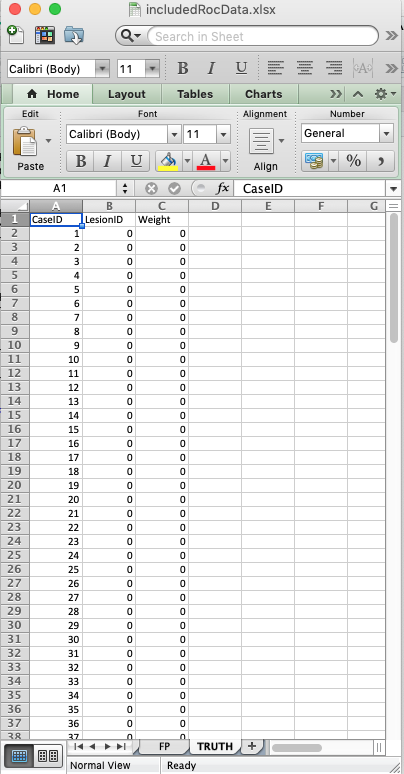
\includegraphics[width=0.4\textwidth,height=\textheight]{images/ROC-Truth-1.png}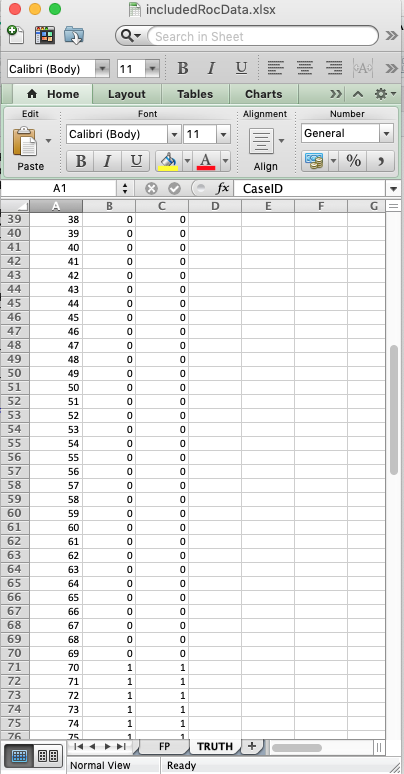
\includegraphics[width=0.4\textwidth,height=\textheight]{images/ROC-Truth-2.png}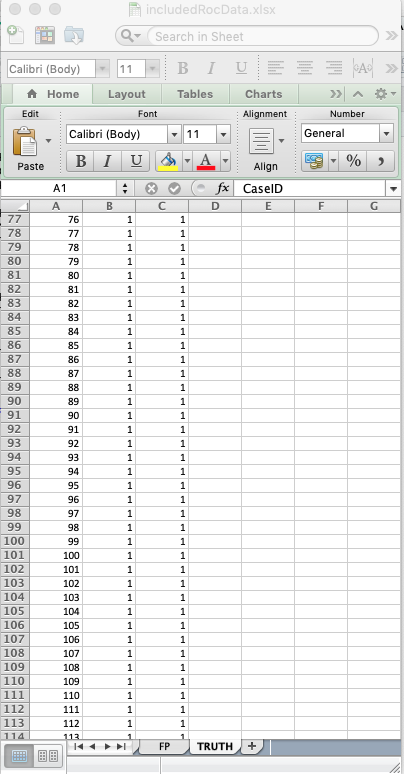
\includegraphics[width=0.4\textwidth,height=\textheight]{images/ROC-Truth-3.png}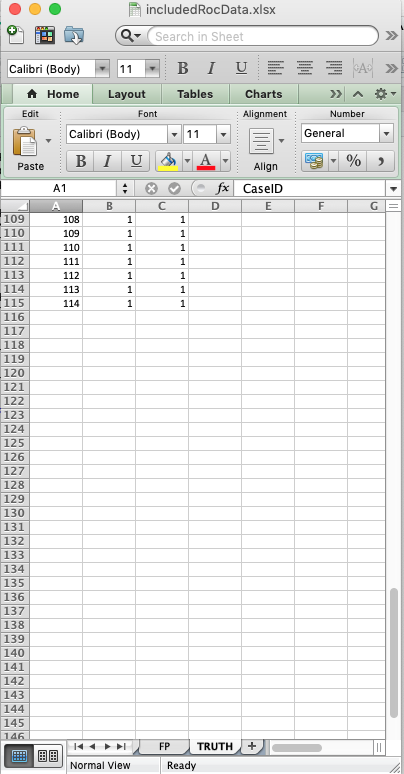
\includegraphics[width=0.4\textwidth,height=\textheight]{images/ROC-Truth-4.png}

\begin{itemize}
\tightlist
\item
  There are 69 non-diseased cases (labeled 1-69) under column \texttt{CaseID}.
\item
  There are 45 diseased cases (labeled 70-114) under column \texttt{CaseID}.\\
\item
  The \texttt{LesionID} field for each non-diseased case (e.g., \texttt{CaseID} = 1) is zero. A zero in this field defines a non-diseased case.
\item
  The \texttt{LesionID} field for each diseased case (e.g., \texttt{CaseID} = 70) is unity. A unit value in this field defines a diseased case.
\item
  The \texttt{Weights} field is irrelevant for ROC datasets. For convenience it is filled with zeroes.
\end{itemize}

\hypertarget{the-fpnl-worksheet-organization}{%
\subsection{The FP/NL worksheet organization}\label{the-fpnl-worksheet-organization}}

The following screen-shots show different parts of the \texttt{FP} worsheet for \texttt{dataset02}.

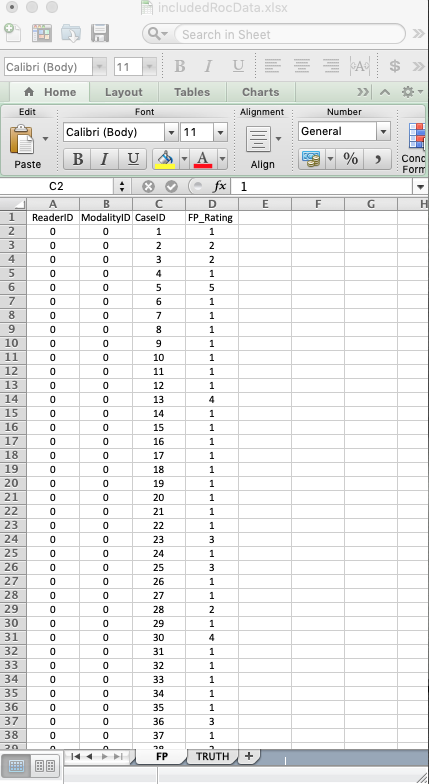
\includegraphics[width=0.4\textwidth,height=\textheight]{images/ROC-FP-1.png}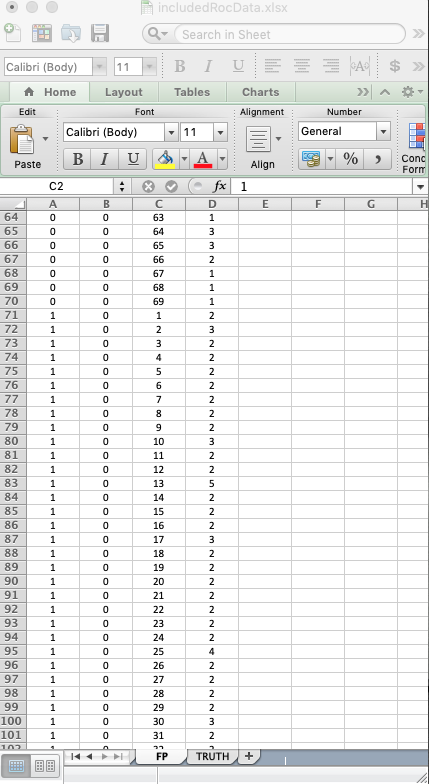
\includegraphics[width=0.4\textwidth,height=\textheight]{images/ROC-FP-2.png}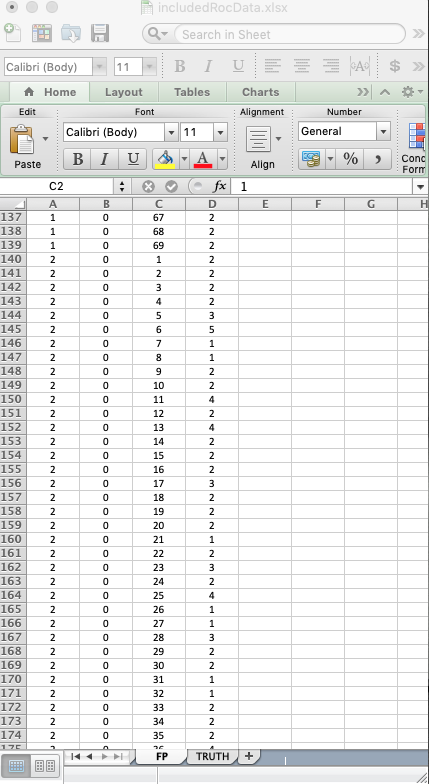
\includegraphics[width=0.4\textwidth,height=\textheight]{images/ROC-FP-3.png}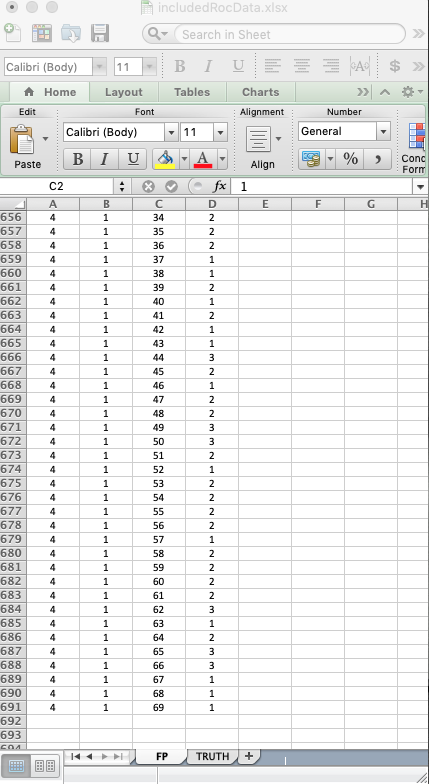
\includegraphics[width=0.4\textwidth,height=\textheight]{images/ROC-FP-5.png}

\begin{itemize}
\tightlist
\item
  The \texttt{FP} (or \texttt{NL}) worksheet lists the ratings of non-diseased cases.
\item
  The \textbf{ModalityID} values range from \texttt{0} to \texttt{1}, corresponding to two treatments.
\item
  The \textbf{ReaderID} values range from \texttt{0} to \texttt{4}, corresponding to five readers.
\item
  The \textbf{CaseID} values range from \texttt{1} to \texttt{69}, corresponding to non-diseased cases \textbf{only}.
\item
  For each reader and treatment, each non-diseased case gets one rating; therefore the length of the column labeled \textbf{FP-Rating} is \textbf{69 x 2 x 5 = 690}.
\item
  The FP ratings tend to be low, there are a lot of ones, fewer twos, even fewer threes, and an ocassional four and a five rating may be found.
\end{itemize}

\hypertarget{the-tpll-worksheet-organization}{%
\subsection{The TP/LL worksheet organization}\label{the-tpll-worksheet-organization}}

The following screen-shots show different parts of the \texttt{FP} worsheet for \texttt{dataset02}.

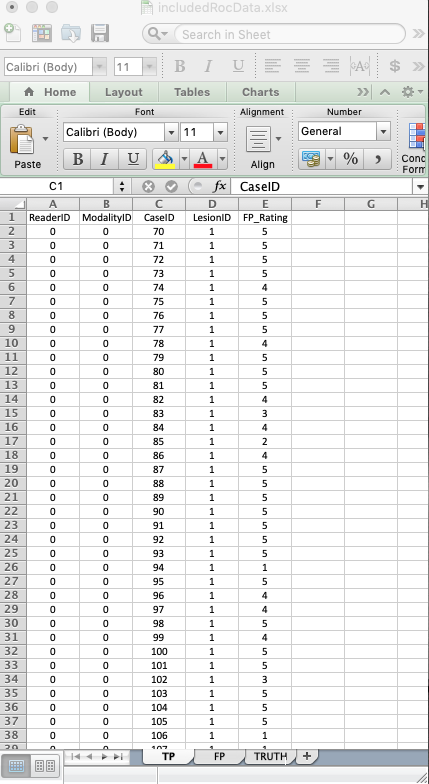
\includegraphics[width=0.4\textwidth,height=\textheight]{images/ROC-TP-1.png}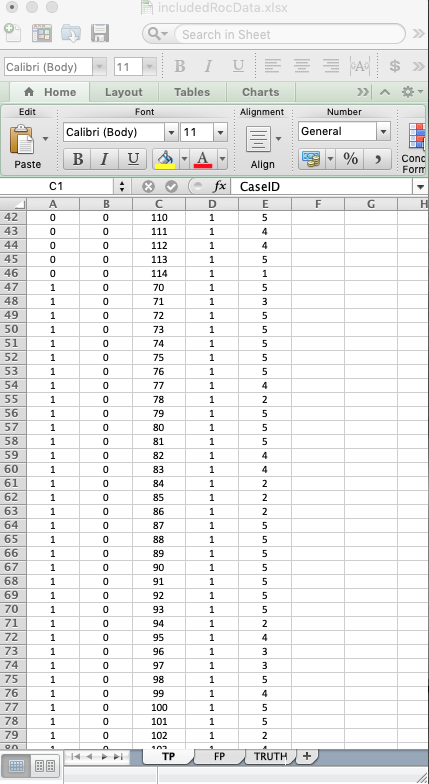
\includegraphics[width=0.4\textwidth,height=\textheight]{images/ROC-TP-2.png}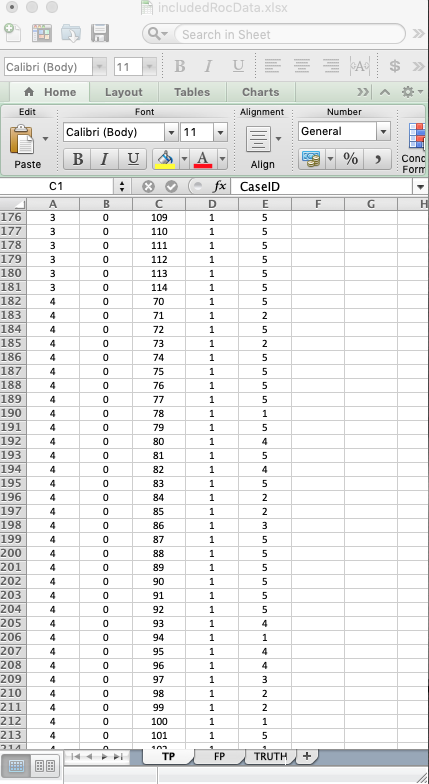
\includegraphics[width=0.4\textwidth,height=\textheight]{images/ROC-TP-3.png}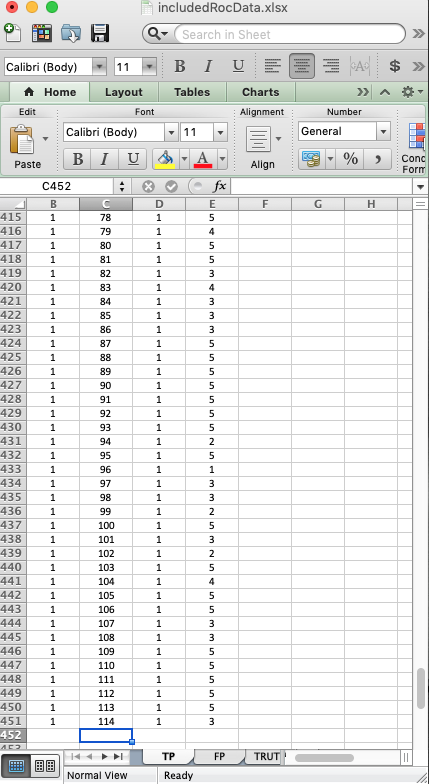
\includegraphics[width=0.4\textwidth,height=\textheight]{images/ROC-TP-4.png}

\begin{itemize}
\tightlist
\item
  The \texttt{TP} (or \texttt{LL}) worksheet lists the ratings of diseased cases.
\item
  The \textbf{ModalityID} values range from \texttt{0} to \texttt{1}, corresponding to two treatments.
\item
  The \textbf{ReaderID} values range from \texttt{0} to \texttt{4}, corresponding to five readers.
\item
  The \textbf{CaseID} values range from \texttt{70} to \texttt{114}, corresponding to diseased cases \textbf{only}.
\item
  For each reader and treatment, each non-diseased case gets one rating; therefore the length of the column labeled \textbf{FP-Rating} is \textbf{45 x 2 x 5 = 450}.
\item
  The TP ratings tend to be high, there are a lot of fives, fewer fours, even fewer threes, and an ocassional two and a one rating may be found.
\end{itemize}

\hypertarget{summary}{%
\section{Summary}\label{summary}}

\begin{itemize}
\tightlist
\item
  Since each case gets one rating, the ROC data structure is relatively easy to visualize. For a single treatment and single reader, all of the information in the dataset can be summarize by a two-row five-column table, with one row listing the number of non-diseased cases rated 1, the number rated two, etc., ending with the number rated five, and a corresponding row for diseased cases. These 10 values contain all of the information contained in the Excel file for the specified treatment and reader. The example below is for treatment \texttt{0} and reader \texttt{0}:
\end{itemize}

\begin{Shaded}
\begin{Highlighting}[]
\NormalTok{nl <-}\StringTok{ }\NormalTok{dataset02}\OperatorTok{$}\NormalTok{NL}
\NormalTok{binnedFpCounts <-}\StringTok{ }\KeywordTok{array}\NormalTok{(}\DecValTok{5}\NormalTok{)}
\ControlFlowTok{for}\NormalTok{ (b }\ControlFlowTok{in} \DecValTok{1}\OperatorTok{:}\DecValTok{5}\NormalTok{) binnedFpCounts[b] <-}\StringTok{ }\KeywordTok{sum}\NormalTok{(nl[}\DecValTok{1}\NormalTok{,}\DecValTok{1}\NormalTok{,}\DecValTok{1}\OperatorTok{:}\NormalTok{K1,}\DecValTok{1}\NormalTok{] }\OperatorTok{==}\StringTok{ }\NormalTok{b)}
\NormalTok{ll <-}\StringTok{ }\NormalTok{dataset02}\OperatorTok{$}\NormalTok{LL}
\NormalTok{binnedTpCounts <-}\StringTok{ }\KeywordTok{array}\NormalTok{(}\DecValTok{5}\NormalTok{)}
\ControlFlowTok{for}\NormalTok{ (b }\ControlFlowTok{in} \DecValTok{1}\OperatorTok{:}\DecValTok{5}\NormalTok{) binnedTpCounts[b] <-}\StringTok{ }\KeywordTok{sum}\NormalTok{(ll[}\DecValTok{1}\NormalTok{,}\DecValTok{1}\NormalTok{,}\DecValTok{1}\OperatorTok{:}\NormalTok{K2,}\DecValTok{1}\NormalTok{] }\OperatorTok{==}\StringTok{ }\NormalTok{b)}
\NormalTok{binnedFpCounts}
\CommentTok{#> [1] 47  9 10  2  1}
\NormalTok{binnedTpCounts}
\CommentTok{#> [1]  4  1  2 10 28}
\KeywordTok{sum}\NormalTok{(binnedFpCounts)}
\CommentTok{#> [1] 69}
\KeywordTok{sum}\NormalTok{(binnedTpCounts)}
\CommentTok{#> [1] 45}
\end{Highlighting}
\end{Shaded}

\begin{itemize}
\tightlist
\item
  The values in \texttt{binnedFpCounts} sum to 69.
\item
  The values in \texttt{binnedTpCounts} sum to 45.
\item
  A similar table is needed for each treatment-reader combination.
\item
  The real value of the Excel format is that it allows generalization to other paradigms where the number of ratings per case is variable.
\end{itemize}

\hypertarget{frocdataformat}{%
\chapter{FROC data format}\label{frocdataformat}}

\hypertarget{introduction-1}{%
\section{Introduction}\label{introduction-1}}

\begin{itemize}
\tightlist
\item
  In the free-response ROC (\textbf{FROC}) paradigm \citep{RN85} the observer's task is to:

  \begin{itemize}
  \tightlist
  \item
    \textbf{mark} (i.e., indicate the location of) and
  \item
    \textbf{rate} (i.e., assign an ordered label representing the degree of suspicion) regions in the image that are perceived as suspicious for presence of disease.
  \item
    Accordingly, FROC data consists of \textbf{mark-rating pairs}, where each mark indicates a region \footnote{In order to avoid confusion with the region-of-interest or ROI-paradigm, I do not like to use the term ROI to describe the marks made by the observer.} that was considered suspicious for presence of a localized lesion and the rating is the corresponding confidence level.
  \item
    The number of mark-rating pairs on any particular case is a-priori unpredictable. It is a non-negative random integer (i.e., 0, 1, 2, \ldots{}) that depends on the case, the reader and the modality. The relatively unstructured nature of FROC data makes FROC paradigm data seemingly more difficult to analyze than ROC paradigm data \footnote{I say ``seemingly'', because the only real difference between ROC and FROC analyses is in the selection of the figure of merit.}.
  \end{itemize}
\item
  By adopting a proximity criterion, each mark is classified by the investigator as a lesion localization (LL) - if it is close to a real lesion - or a non-lesion localization (NL) otherwise.
\item
  The rating can be an integer or quasi- continuous (e.g., 0 -- 100), or a floating point value, as long as higher numbers represent greater confidence in presence of one or more lesions in the ROI \footnote{As with the ROC paradigm, the directionaliy of the rating is not a limitation.}.
\item
  For human observer studies a 4 or 5-point rating scale is recommended:

  \begin{itemize}
  \tightlist
  \item
    1: Very low, but finite possibility that the region is diseased.
  \item
    2: Low possibility that the region is diseased.
  \item
    3: Moderate possibility that the region is diseased.
  \item
    4: High possibility that the region is diseased.
  \item
    5: Very high possibility that the region is diseased.
  \end{itemize}
\item
  The actual adjectives used to describe the labels are unimportant. What is important is the ordering of the labels and that the observer holds them relatively constant for the duration of the study. More allowed ratings, provided the observer can work with them, leads to greater definition of the relevant empirical operating curves (to be introduced later).
\item
  With algorithmic readers, e.g., computer aided detection (CAD) algorithms, a floating point rating, if possible, should be retained.
\item
  In the most common study design, termed multiple-reader multiple-case (\textbf{MRMC}), the rating collection procedure is repeated for all cases, treatments and readers.
\end{itemize}

\hypertarget{an-actual-mrmc-froc-dataset}{%
\section{An actual MRMC FROC dataset}\label{an-actual-mrmc-froc-dataset}}

An actual MRMC FROC dataset is included as \texttt{dataset04} \citep{RN1882}. It has the following structure:

\begin{Shaded}
\begin{Highlighting}[]
\KeywordTok{str}\NormalTok{(dataset04)}
\CommentTok{#> List of 8}
\CommentTok{#>  $ NL          : num [1:5, 1:4, 1:200, 1:7] -Inf -Inf 1 -Inf -Inf ...}
\CommentTok{#>  $ LL          : num [1:5, 1:4, 1:100, 1:3] 4 5 4 5 4 3 5 4 4 3 ...}
\CommentTok{#>  $ lesionNum   : int [1:100] 1 1 1 1 1 1 1 1 1 1 ...}
\CommentTok{#>  $ lesionID    : num [1:100, 1:3] 1 1 1 1 1 1 1 1 1 1 ...}
\CommentTok{#>  $ lesionWeight: num [1:100, 1:3] 1 1 1 1 1 1 1 1 1 1 ...}
\CommentTok{#>  $ dataType    : chr "FROC"}
\CommentTok{#>  $ modalityID  : Named chr [1:5] "1" "2" "3" "4" ...}
\CommentTok{#>   ..- attr(*, "names")= chr [1:5] "1" "2" "3" "4" ...}
\CommentTok{#>  $ readerID    : Named chr [1:4] "1" "3" "4" "5"}
\CommentTok{#>   ..- attr(*, "names")= chr [1:4] "1" "3" "4" "5"}
\end{Highlighting}
\end{Shaded}

The \texttt{dataset} structure is a \texttt{list} variable with 8 members.

\hypertarget{the-nl-aand-ll-list-members}{%
\subsection{\texorpdfstring{The \texttt{NL} aand \texttt{LL} list members}{The NL aand LL list members}}\label{the-nl-aand-ll-list-members}}

\begin{itemize}
\tightlist
\item
  Ratings of actually non-diseased regions are stored in the \texttt{NL} list member.
\item
  Ratings of actually diseased regions are stored in the \texttt{LL} list member.
\item
  \texttt{dataset04} corresponds to 5-treatments and 4-readers (the lengths of the first and second dimensions, respectively, of the \texttt{NL} and \texttt{LL} arrays).
\end{itemize}

\hypertarget{the-lesionnum-list-member}{%
\subsection{\texorpdfstring{The \texttt{lesionNum} list member}{The lesionNum list member}}\label{the-lesionnum-list-member}}

\begin{itemize}
\tightlist
\item
  The \texttt{lesionNum} list member is an array of length 100 filled with integers ranging from 1 to 3, the latter being the maximum number of actual lesions per case in \texttt{dataset04}. The length of this array equals the number of diseased cases, 100 in the current example. The contents of \texttt{lesionNum} are shown below:
\end{itemize}

\begin{Shaded}
\begin{Highlighting}[]
\NormalTok{dataset04}\OperatorTok{$}\NormalTok{lesionNum[}\DecValTok{1}\OperatorTok{:}\DecValTok{20}\NormalTok{]}
\CommentTok{#>  [1] 1 1 1 1 1 1 1 1 1 1 1 1 1 1 1 1 1 1 1 1}
\NormalTok{dataset04}\OperatorTok{$}\NormalTok{lesionNum[}\DecValTok{21}\OperatorTok{:}\DecValTok{40}\NormalTok{]}
\CommentTok{#>  [1] 1 1 1 1 1 1 1 1 1 1 1 1 1 1 1 1 1 1 1 1}
\NormalTok{dataset04}\OperatorTok{$}\NormalTok{lesionNum[}\DecValTok{41}\OperatorTok{:}\DecValTok{60}\NormalTok{]}
\CommentTok{#>  [1] 1 1 1 1 1 1 1 1 1 1 1 1 1 1 1 2 2 1 1 2}
\NormalTok{dataset04}\OperatorTok{$}\NormalTok{lesionNum[}\DecValTok{61}\OperatorTok{:}\DecValTok{80}\NormalTok{]}
\CommentTok{#>  [1] 1 1 1 1 1 1 1 1 2 2 1 1 1 2 2 2 2 2 2 1}
\NormalTok{dataset04}\OperatorTok{$}\NormalTok{lesionNum[}\DecValTok{81}\OperatorTok{:}\DecValTok{100}\NormalTok{]}
\CommentTok{#>  [1] 2 2 2 2 3 2 2 2 2 2 3 3 3 3 3 3 3 3 3 3}
\end{Highlighting}
\end{Shaded}

\begin{itemize}
\tightlist
\item
  The above entries tell us that while most cases contain only one lesion each, some contain 2 or even 3 lesions per case.
\end{itemize}

\hypertarget{the-lesionid-list-member}{%
\subsection{\texorpdfstring{The \texttt{lesionID} list member}{The lesionID list member}}\label{the-lesionid-list-member}}

\begin{itemize}
\tightlist
\item
  The \texttt{lesionID} list member is a \texttt{{[}100\ x\ 3{]}} array.
\item
  Essentially it establishes a way of distinguishing between different lesions on a case by naming them, or what amounts to the same thing, by labeling them.
\item
  The problem of distinguishing between different lesions on a case is peculiar to the FROC paradigm. With only one conceptual lesion per diseased case, the ROC paradigm does not face this problem.
\item
  The second dimension of this array indicates that there is at least one diseased case with three lesions.
\end{itemize}

\begin{Shaded}
\begin{Highlighting}[]
\NormalTok{dataset04}\OperatorTok{$}\NormalTok{lesionID[}\DecValTok{1}\OperatorTok{:}\DecValTok{10}\NormalTok{,]}
\CommentTok{#>       [,1] [,2] [,3]}
\CommentTok{#>  [1,]    1 -Inf -Inf}
\CommentTok{#>  [2,]    1 -Inf -Inf}
\CommentTok{#>  [3,]    1 -Inf -Inf}
\CommentTok{#>  [4,]    1 -Inf -Inf}
\CommentTok{#>  [5,]    1 -Inf -Inf}
\CommentTok{#>  [6,]    1 -Inf -Inf}
\CommentTok{#>  [7,]    1 -Inf -Inf}
\CommentTok{#>  [8,]    1 -Inf -Inf}
\CommentTok{#>  [9,]    1 -Inf -Inf}
\CommentTok{#> [10,]    1 -Inf -Inf}
\end{Highlighting}
\end{Shaded}

\begin{itemize}
\tightlist
\item
  This indicates that the first ten diseased cases contain one lesion each.
\item
  The lesion on case 1 is \textbf{labeled} by the value 1. The \texttt{-Inf} denote missing values. Since there is only one lesion, the placeholders for the second or third lesion (not present on this case, but needed to hold lesion labels in other cases) need to be filled with negative infinites.
\item
  The following example may help clarify this point.
\end{itemize}

\begin{Shaded}
\begin{Highlighting}[]
\NormalTok{dataset04}\OperatorTok{$}\NormalTok{lesionID[}\DecValTok{90}\OperatorTok{:}\DecValTok{100}\NormalTok{,]}
\CommentTok{#>       [,1] [,2] [,3]}
\CommentTok{#>  [1,]    1    2 -Inf}
\CommentTok{#>  [2,]    1    2    3}
\CommentTok{#>  [3,]    1    2    3}
\CommentTok{#>  [4,]    1    2    3}
\CommentTok{#>  [5,]    1    2    3}
\CommentTok{#>  [6,]    1    2    3}
\CommentTok{#>  [7,]    1    2    3}
\CommentTok{#>  [8,]    1    2    3}
\CommentTok{#>  [9,]    1    2    3}
\CommentTok{#> [10,]    1    2    3}
\CommentTok{#> [11,]    1    2    3}
\end{Highlighting}
\end{Shaded}

\begin{itemize}
\tightlist
\item
  Diseased case 90 has two lesions, labeled 1 and 2 respectively.
\item
  The key point is this: each lesion on a case has a distinct \emph{name}. Just as each case has to have a distinct name (i.e., label), each lesion within a (diseased) case has to have a distinct name.
\item
  When an observer assigns a rating to a particular lesion on a casee, the experimenter needs to record this information correctly.
\item
  For example, if the lesion with \texttt{lesionID\ =\ 1} is marked and rated a particular value, this value needs to be entered in the spread-sheet as belonging to the lesion named \texttt{lesionID\ =\ 1}.
\item
  The \texttt{TP/LL} worksheet has a \texttt{lesionID} column. \footnote{Since the ROC paradigm does not allow multiple lesions per case, each diseased case conceptually containing only one lesion, the distinction between different \texttt{lesionID} values on the same diseased case does not arise.}
\item
  The distinction implied by different \texttt{lesionID} values is important if the lesion weights are unequal.\footnote{For equally weighted lesions, the name distinction implied by \texttt{lesionID} is not important, but then the analysis would only be valid for equally weighted lesions.}
\end{itemize}

\hypertarget{the-lesionweight-list-member}{%
\subsection{\texorpdfstring{The \texttt{LesionWeight} list member}{The LesionWeight list member}}\label{the-lesionweight-list-member}}

\begin{itemize}
\tightlist
\item
  The \texttt{LesionWeight} list member is also a \texttt{{[}100\ x\ 3{]}} array filled with values that add up to unity for each case. The meaning of lesion weights is dicussed in here: \citep{RN1385, RN1966, RN2680}
\item
  Briefly, the lesion weights are the clinical importance of detecting the lesion.
\item
  As an example, a highly visible lesion might have low clinical significance if it is likely to be benign, and it would be characterized by a lower weight than a less visible but more deadly lesion on the same case.
\item
  In order to give each case equal importance, the weights must sum to one.
\item
  In the current example, see below, the lesions are equally weighted.
\item
  The choice of weights is a clinical consideration, determined by the costs and benefits of missing or finding the lesion. Lacking this information, which is the most common scenario, it makes sense to weight the lesions equally.
\item
  On a case one one lesion, \texttt{lesionWeight\ =\ 1}, and the other lesionWeights are assigned negative infinity values.
\item
  On a case with two lesions, \texttt{lesionWeight\ =\ 0.5} for the first two lesions, and the third weight is assigned the negative infinity value.
\item
  On a case with three lesions, \texttt{lesionWeight\ =\ 0.3333} for the lesions.
\item
  Rather than assign these values manually, set the Weight column of the Truth worksheet to zeroes. Then the software automatically assigns equal weights when the Excel sheet is read.
\end{itemize}

\begin{Shaded}
\begin{Highlighting}[]
\NormalTok{dataset04}\OperatorTok{$}\NormalTok{lesionWeight[}\DecValTok{1}\OperatorTok{:}\DecValTok{20}\NormalTok{,]}
\CommentTok{#>       [,1] [,2] [,3]}
\CommentTok{#>  [1,]    1 -Inf -Inf}
\CommentTok{#>  [2,]    1 -Inf -Inf}
\CommentTok{#>  [3,]    1 -Inf -Inf}
\CommentTok{#>  [4,]    1 -Inf -Inf}
\CommentTok{#>  [5,]    1 -Inf -Inf}
\CommentTok{#>  [6,]    1 -Inf -Inf}
\CommentTok{#>  [7,]    1 -Inf -Inf}
\CommentTok{#>  [8,]    1 -Inf -Inf}
\CommentTok{#>  [9,]    1 -Inf -Inf}
\CommentTok{#> [10,]    1 -Inf -Inf}
\CommentTok{#> [11,]    1 -Inf -Inf}
\CommentTok{#> [12,]    1 -Inf -Inf}
\CommentTok{#> [13,]    1 -Inf -Inf}
\CommentTok{#> [14,]    1 -Inf -Inf}
\CommentTok{#> [15,]    1 -Inf -Inf}
\CommentTok{#> [16,]    1 -Inf -Inf}
\CommentTok{#> [17,]    1 -Inf -Inf}
\CommentTok{#> [18,]    1 -Inf -Inf}
\CommentTok{#> [19,]    1 -Inf -Inf}
\CommentTok{#> [20,]    1 -Inf -Inf}
\NormalTok{dataset04}\OperatorTok{$}\NormalTok{lesionWeight[}\DecValTok{21}\OperatorTok{:}\DecValTok{40}\NormalTok{,]}
\CommentTok{#>       [,1] [,2] [,3]}
\CommentTok{#>  [1,]    1 -Inf -Inf}
\CommentTok{#>  [2,]    1 -Inf -Inf}
\CommentTok{#>  [3,]    1 -Inf -Inf}
\CommentTok{#>  [4,]    1 -Inf -Inf}
\CommentTok{#>  [5,]    1 -Inf -Inf}
\CommentTok{#>  [6,]    1 -Inf -Inf}
\CommentTok{#>  [7,]    1 -Inf -Inf}
\CommentTok{#>  [8,]    1 -Inf -Inf}
\CommentTok{#>  [9,]    1 -Inf -Inf}
\CommentTok{#> [10,]    1 -Inf -Inf}
\CommentTok{#> [11,]    1 -Inf -Inf}
\CommentTok{#> [12,]    1 -Inf -Inf}
\CommentTok{#> [13,]    1 -Inf -Inf}
\CommentTok{#> [14,]    1 -Inf -Inf}
\CommentTok{#> [15,]    1 -Inf -Inf}
\CommentTok{#> [16,]    1 -Inf -Inf}
\CommentTok{#> [17,]    1 -Inf -Inf}
\CommentTok{#> [18,]    1 -Inf -Inf}
\CommentTok{#> [19,]    1 -Inf -Inf}
\CommentTok{#> [20,]    1 -Inf -Inf}
\NormalTok{dataset04}\OperatorTok{$}\NormalTok{lesionWeight[}\DecValTok{41}\OperatorTok{:}\DecValTok{60}\NormalTok{,]}
\CommentTok{#>       [,1] [,2] [,3]}
\CommentTok{#>  [1,]  1.0 -Inf -Inf}
\CommentTok{#>  [2,]  1.0 -Inf -Inf}
\CommentTok{#>  [3,]  1.0 -Inf -Inf}
\CommentTok{#>  [4,]  1.0 -Inf -Inf}
\CommentTok{#>  [5,]  1.0 -Inf -Inf}
\CommentTok{#>  [6,]  1.0 -Inf -Inf}
\CommentTok{#>  [7,]  1.0 -Inf -Inf}
\CommentTok{#>  [8,]  1.0 -Inf -Inf}
\CommentTok{#>  [9,]  1.0 -Inf -Inf}
\CommentTok{#> [10,]  1.0 -Inf -Inf}
\CommentTok{#> [11,]  1.0 -Inf -Inf}
\CommentTok{#> [12,]  1.0 -Inf -Inf}
\CommentTok{#> [13,]  1.0 -Inf -Inf}
\CommentTok{#> [14,]  1.0 -Inf -Inf}
\CommentTok{#> [15,]  1.0 -Inf -Inf}
\CommentTok{#> [16,]  0.5  0.5 -Inf}
\CommentTok{#> [17,]  0.5  0.5 -Inf}
\CommentTok{#> [18,]  1.0 -Inf -Inf}
\CommentTok{#> [19,]  1.0 -Inf -Inf}
\CommentTok{#> [20,]  0.5  0.5 -Inf}
\NormalTok{dataset04}\OperatorTok{$}\NormalTok{lesionWeight[}\DecValTok{61}\OperatorTok{:}\DecValTok{80}\NormalTok{,]}
\CommentTok{#>       [,1] [,2] [,3]}
\CommentTok{#>  [1,]  1.0 -Inf -Inf}
\CommentTok{#>  [2,]  1.0 -Inf -Inf}
\CommentTok{#>  [3,]  1.0 -Inf -Inf}
\CommentTok{#>  [4,]  1.0 -Inf -Inf}
\CommentTok{#>  [5,]  1.0 -Inf -Inf}
\CommentTok{#>  [6,]  1.0 -Inf -Inf}
\CommentTok{#>  [7,]  1.0 -Inf -Inf}
\CommentTok{#>  [8,]  1.0 -Inf -Inf}
\CommentTok{#>  [9,]  0.5  0.5 -Inf}
\CommentTok{#> [10,]  0.5  0.5 -Inf}
\CommentTok{#> [11,]  1.0 -Inf -Inf}
\CommentTok{#> [12,]  1.0 -Inf -Inf}
\CommentTok{#> [13,]  1.0 -Inf -Inf}
\CommentTok{#> [14,]  0.5  0.5 -Inf}
\CommentTok{#> [15,]  0.5  0.5 -Inf}
\CommentTok{#> [16,]  0.5  0.5 -Inf}
\CommentTok{#> [17,]  0.5  0.5 -Inf}
\CommentTok{#> [18,]  0.5  0.5 -Inf}
\CommentTok{#> [19,]  0.5  0.5 -Inf}
\CommentTok{#> [20,]  1.0 -Inf -Inf}
\NormalTok{dataset04}\OperatorTok{$}\NormalTok{lesionWeight[}\DecValTok{81}\OperatorTok{:}\DecValTok{100}\NormalTok{,]}
\CommentTok{#>            [,1]      [,2]      [,3]}
\CommentTok{#>  [1,] 0.5000000 0.5000000      -Inf}
\CommentTok{#>  [2,] 0.5000000 0.5000000      -Inf}
\CommentTok{#>  [3,] 0.5000000 0.5000000      -Inf}
\CommentTok{#>  [4,] 0.5000000 0.5000000      -Inf}
\CommentTok{#>  [5,] 0.3333333 0.3333333 0.3333333}
\CommentTok{#>  [6,] 0.5000000 0.5000000      -Inf}
\CommentTok{#>  [7,] 0.5000000 0.5000000      -Inf}
\CommentTok{#>  [8,] 0.5000000 0.5000000      -Inf}
\CommentTok{#>  [9,] 0.5000000 0.5000000      -Inf}
\CommentTok{#> [10,] 0.5000000 0.5000000      -Inf}
\CommentTok{#> [11,] 0.3333333 0.3333333 0.3333333}
\CommentTok{#> [12,] 0.3333333 0.3333333 0.3333333}
\CommentTok{#> [13,] 0.3333333 0.3333333 0.3333333}
\CommentTok{#> [14,] 0.3333333 0.3333333 0.3333333}
\CommentTok{#> [15,] 0.3333333 0.3333333 0.3333333}
\CommentTok{#> [16,] 0.3333333 0.3333333 0.3333333}
\CommentTok{#> [17,] 0.3333333 0.3333333 0.3333333}
\CommentTok{#> [18,] 0.3333333 0.3333333 0.3333333}
\CommentTok{#> [19,] 0.3333333 0.3333333 0.3333333}
\CommentTok{#> [20,] 0.3333333 0.3333333 0.3333333}
\end{Highlighting}
\end{Shaded}

\hypertarget{the-datatype-list-member}{%
\subsection{\texorpdfstring{The \texttt{dataType} list member}{The dataType list member}}\label{the-datatype-list-member}}

\begin{itemize}
\tightlist
\item
  The \texttt{dataType} list member equals the string \texttt{"FROC"}, identifying \texttt{dataset04} as an FROC dataset.
\end{itemize}

Examination of the output reveals that:

\begin{itemize}
\tightlist
\item
  Location-level ratings of non-diseased regions are stored in the \texttt{NL} list member.
\item
  Location-level ratings of diseased regions are stored in the \texttt{LL} list member.
\end{itemize}

\hypertarget{details-of-the-modalityid-and-readerid-list-members-1}{%
\subsection{\texorpdfstring{Details of the \texttt{modalityID} and \texttt{readerID} list members}{Details of the modalityID and readerID list members}}\label{details-of-the-modalityid-and-readerid-list-members-1}}

\begin{itemize}
\tightlist
\item
  The names of the treatments are in the \texttt{modalityID} list member:
\end{itemize}

\begin{Shaded}
\begin{Highlighting}[]
\KeywordTok{attributes}\NormalTok{(dataset04}\OperatorTok{$}\NormalTok{modalityID)}
\CommentTok{#> $names}
\CommentTok{#> [1] "1" "2" "3" "4" "5"}
\end{Highlighting}
\end{Shaded}

\begin{itemize}
\item
  For example, the name of the second treatment is \texttt{"2"}. The names can be longer strings, but use of very long string names may mess up the output formats of the analysis report.
\item
  The names of the readers are in the \texttt{readerID} array:
\end{itemize}

\begin{Shaded}
\begin{Highlighting}[]
\KeywordTok{attributes}\NormalTok{(dataset04}\OperatorTok{$}\NormalTok{readerID)}
\CommentTok{#> $names}
\CommentTok{#> [1] "1" "3" "4" "5"}
\end{Highlighting}
\end{Shaded}

For example, the name of the second reader is \texttt{"3"}. Apparently reader \texttt{"2"} ``dropped out'' of the study. A similar caveat regarding long reader names applies.

\hypertarget{details-of-the-nl-and-ll-list-members-1}{%
\subsection{\texorpdfstring{Details of the \texttt{NL} and \texttt{LL} list members}{Details of the NL and LL list members}}\label{details-of-the-nl-and-ll-list-members-1}}

\begin{itemize}
\tightlist
\item
  For either \texttt{NL} or \texttt{LL} list members, the fourth dimension can have length greater than unity.
\item
  For the \texttt{NL} list member \textbf{this length is determined by the treatment-reader-case combination yielding the most \texttt{NL} marks per case}.
\item
  For the \texttt{LL} list member \textbf{this length is determined by the case with the most true lesions}.
\item
  \texttt{dataset02} is a 2-treatment 5-reader dataset (the lengths of the first and second dimensions, respectively, of the \texttt{NL} and \texttt{LL} list members).
\end{itemize}

\hypertarget{numbers-of-non-diseased-and-diseased-cases-1}{%
\subsection{Numbers of non-diseased and diseased cases}\label{numbers-of-non-diseased-and-diseased-cases-1}}

\begin{Shaded}
\begin{Highlighting}[]
\KeywordTok{length}\NormalTok{(dataset04}\OperatorTok{$}\NormalTok{NL[}\DecValTok{1}\NormalTok{,}\DecValTok{1}\NormalTok{,,}\DecValTok{1}\NormalTok{])}
\CommentTok{#> [1] 200}
\KeywordTok{length}\NormalTok{(dataset04}\OperatorTok{$}\NormalTok{LL[}\DecValTok{1}\NormalTok{,}\DecValTok{1}\NormalTok{,,}\DecValTok{1}\NormalTok{])}
\CommentTok{#> [1] 100}
\end{Highlighting}
\end{Shaded}

\begin{itemize}
\tightlist
\item
  The third dimension of the \texttt{NL} array is the total number of \textbf{all} cases, i.e., 200, and the third dimension of the \texttt{LL} array, i.e., 100, is the total number of diseased cases.
\item
  Subtracting the number of diseased cases from the number of all cases yields the number of non-diseased cases.
\item
  Therefore, in this dataset, there are 100 diseased cases and 100 non-diseased cases.
\end{itemize}

\hypertarget{why-dimension-the-nl-array-for-the-total-number-of-cases-1}{%
\subsection{\texorpdfstring{Why dimension the \texttt{NL} array for the total number of cases?}{Why dimension the NL array for the total number of cases?}}\label{why-dimension-the-nl-array-for-the-total-number-of-cases-1}}

\begin{itemize}
\tightlist
\item
  Because, in addition to \texttt{LLs}, \texttt{NLs} are possible on diseased cases.
\item
  Only \texttt{LLs} are possible on diseased cases.
\item
  Only \texttt{NLs} are possible on non-diseased cases.
\item
  The missing values are filled in with \texttt{-Inf}.
\end{itemize}

\hypertarget{ratings-on-a-non-diseased-case-1}{%
\subsection{Ratings on a non-diseased case}\label{ratings-on-a-non-diseased-case-1}}

\begin{itemize}
\tightlist
\item
  For treatment 1, reader 1 and case 1 (the first non-diseased case), the NL ratings are:
\end{itemize}

\begin{Shaded}
\begin{Highlighting}[]
\NormalTok{dataset04}\OperatorTok{$}\NormalTok{NL[}\DecValTok{1}\NormalTok{,}\DecValTok{1}\NormalTok{,}\DecValTok{1}\NormalTok{,]}
\CommentTok{#> [1] -Inf -Inf -Inf -Inf -Inf -Inf -Inf}
\end{Highlighting}
\end{Shaded}

\hypertarget{the-meaning-of-a-negative-infinity-rating}{%
\subsubsection{The meaning of a negative infinity rating}\label{the-meaning-of-a-negative-infinity-rating}}

\begin{itemize}
\tightlist
\item
  Obviously, a real rating cannot be negative infinity \footnote{If an observer is so highly confident in the \emph{absence} of a localized lesion, he will simply \emph{not mark} the location in question; if he did, then, logically, he should mark \emph{all} areas in the image that are definitely not lesions; in the FROC paradigm only regions with a reasonable degree of suspicion are marked. The radiologist only wishes to draw attention to regions that are reasonably suspicious; the definition of ``reasonable'' is determined by clinical considerations.}. This value is reserved for \textbf{missing ratings}, and more generally, \textbf{missing marks} \footnote{Since there is a one-to-one correspondence between marks and ratings.}. For example, since all values in the above code chunk are negative infinities, this means this treatment-reader-case combination did not yield any mark-rating pairs. This possibility, alluded to above, is only possible with FROC data. All other paradigms (ROC, LROC and ROI) yield at least one rating per case.
\item
  The length of the fourth dimension of the \texttt{NL} array is determined by that treatment-reader-case combination yielding the maximum number of \texttt{NLs}. Consider the following chunk:
\end{itemize}

\begin{Shaded}
\begin{Highlighting}[]
\ControlFlowTok{for}\NormalTok{ (i }\ControlFlowTok{in} \DecValTok{1}\OperatorTok{:}\DecValTok{5}\NormalTok{) }
  \ControlFlowTok{for}\NormalTok{ (j }\ControlFlowTok{in} \DecValTok{1}\OperatorTok{:}\DecValTok{4}\NormalTok{) }
    \ControlFlowTok{for}\NormalTok{ (k }\ControlFlowTok{in} \DecValTok{1}\OperatorTok{:}\DecValTok{200}\NormalTok{) }
      \ControlFlowTok{if}\NormalTok{ (}\KeywordTok{all}\NormalTok{(dataset04}\OperatorTok{$}\NormalTok{NL[i,j,k,] }\OperatorTok{!=}\StringTok{ }\OperatorTok{-}\OtherTok{Inf}\NormalTok{)) }
        \KeywordTok{cat}\NormalTok{(i, j, k, }\KeywordTok{all}\NormalTok{(dataset04}\OperatorTok{$}\NormalTok{NL[i,j,k,] }\OperatorTok{!=}\StringTok{ }\OperatorTok{-}\OtherTok{Inf}\NormalTok{),}\StringTok{"}\CharTok{\textbackslash{}n}\StringTok{"}\NormalTok{)}
\CommentTok{#> 5 4 192 TRUE}
\end{Highlighting}
\end{Shaded}

\begin{itemize}
\tightlist
\item
  This shows that the fourth dimension of the \texttt{NL} array has to be of length 7 because \emph{one, and only reader}, specifically reader ``4'', made 7 \texttt{NL} marks on a diseased case in treatment ``5''!
\end{itemize}

\hypertarget{ratings-on-a-diseased-case-1}{%
\subsubsection{Ratings on a diseased case}\label{ratings-on-a-diseased-case-1}}

Unlike non-diseased cases, diseased cases can have both \texttt{NL} and \texttt{LL} ratings.

\begin{itemize}
\tightlist
\item
  For treatment 1, reader 1, case 51 (the 1st diseased case) the NL ratings are:
\end{itemize}

\begin{Shaded}
\begin{Highlighting}[]
\NormalTok{dataset04}\OperatorTok{$}\NormalTok{NL[}\DecValTok{1}\NormalTok{,}\DecValTok{1}\NormalTok{,}\DecValTok{51}\NormalTok{,]}
\CommentTok{#> [1] -Inf -Inf -Inf -Inf -Inf -Inf -Inf}
\NormalTok{dataset04}\OperatorTok{$}\NormalTok{lesionNum[}\DecValTok{1}\NormalTok{]}
\CommentTok{#> [1] 1}
\NormalTok{dataset04}\OperatorTok{$}\NormalTok{LL[}\DecValTok{1}\NormalTok{,}\DecValTok{1}\NormalTok{,}\DecValTok{1}\NormalTok{,]}
\CommentTok{#> [1]    4 -Inf -Inf}
\KeywordTok{mean}\NormalTok{(}\KeywordTok{is.finite}\NormalTok{(dataset04}\OperatorTok{$}\NormalTok{LL))}
\CommentTok{#> [1] 0.3043333}
\end{Highlighting}
\end{Shaded}

. There are only two finite values because this case has two ROI-level-abnormal regions, and 2 plus 2 makes for the assumed 4-regions per case. The corresponding \texttt{\$lesionNum} field is 1.

\begin{Shaded}
\begin{Highlighting}[]
\KeywordTok{mean}\NormalTok{(}\KeywordTok{is.finite}\NormalTok{(dataset04}\OperatorTok{$}\NormalTok{NL[,,}\DecValTok{1}\OperatorTok{:}\DecValTok{50}\NormalTok{,]))}
\CommentTok{#> [1] 0.05942857}
\NormalTok{dataset04}\OperatorTok{$}\NormalTok{NL[}\DecValTok{1}\NormalTok{,}\DecValTok{1}\NormalTok{,}\DecValTok{51}\NormalTok{,]}
\CommentTok{#> [1] -Inf -Inf -Inf -Inf -Inf -Inf -Inf}
\NormalTok{dataset04}\OperatorTok{$}\NormalTok{lesionNum[}\DecValTok{1}\NormalTok{]}
\CommentTok{#> [1] 1}
\NormalTok{dataset04}\OperatorTok{$}\NormalTok{LL[}\DecValTok{1}\NormalTok{,}\DecValTok{1}\NormalTok{,}\DecValTok{1}\NormalTok{,]}
\CommentTok{#> [1]    4 -Inf -Inf}
\KeywordTok{mean}\NormalTok{(}\KeywordTok{is.finite}\NormalTok{(dataset04}\OperatorTok{$}\NormalTok{LL))}
\CommentTok{#> [1] 0.3043333}
\end{Highlighting}
\end{Shaded}

\begin{Shaded}
\begin{Highlighting}[]
\KeywordTok{mean}\NormalTok{(}\KeywordTok{is.finite}\NormalTok{(dataset04}\OperatorTok{$}\NormalTok{NL[,,}\DecValTok{1}\OperatorTok{:}\DecValTok{50}\NormalTok{,]))}
\CommentTok{#> [1] 0.05942857}
\NormalTok{dataset04}\OperatorTok{$}\NormalTok{NL[}\DecValTok{1}\NormalTok{,}\DecValTok{1}\NormalTok{,}\DecValTok{51}\NormalTok{,]}
\CommentTok{#> [1] -Inf -Inf -Inf -Inf -Inf -Inf -Inf}
\NormalTok{dataset04}\OperatorTok{$}\NormalTok{lesionNum[}\DecValTok{1}\NormalTok{]}
\CommentTok{#> [1] 1}
\NormalTok{dataset04}\OperatorTok{$}\NormalTok{LL[}\DecValTok{1}\NormalTok{,}\DecValTok{1}\NormalTok{,}\DecValTok{1}\NormalTok{,]}
\CommentTok{#> [1]    4 -Inf -Inf}
\KeywordTok{mean}\NormalTok{(}\KeywordTok{is.finite}\NormalTok{(dataset04}\OperatorTok{$}\NormalTok{LL))}
\CommentTok{#> [1] 0.3043333}
\end{Highlighting}
\end{Shaded}

\begin{itemize}
\tightlist
\item
  The ratings of the 2 \texttt{LLs} on this case are 4. The mean rating over all \texttt{LLs} (in all treatments and readers) is 3.6785323.
\end{itemize}

\begin{Shaded}
\begin{Highlighting}[]
\KeywordTok{mean}\NormalTok{(}\KeywordTok{is.finite}\NormalTok{(dataset04}\OperatorTok{$}\NormalTok{NL[,,}\DecValTok{1}\OperatorTok{:}\DecValTok{50}\NormalTok{,]))}
\CommentTok{#> [1] 0.05942857}
\NormalTok{dataset04}\OperatorTok{$}\NormalTok{NL[}\DecValTok{1}\NormalTok{,}\DecValTok{1}\NormalTok{,}\DecValTok{51}\NormalTok{,]}
\CommentTok{#> [1] -Inf -Inf -Inf -Inf -Inf -Inf -Inf}
\NormalTok{dataset04}\OperatorTok{$}\NormalTok{lesionNum[}\DecValTok{1}\NormalTok{]}
\CommentTok{#> [1] 1}
\NormalTok{dataset04}\OperatorTok{$}\NormalTok{LL[}\DecValTok{1}\NormalTok{,}\DecValTok{1}\NormalTok{,}\DecValTok{1}\NormalTok{,]}
\CommentTok{#> [1]    4 -Inf -Inf}
\KeywordTok{mean}\NormalTok{(}\KeywordTok{is.finite}\NormalTok{(dataset04}\OperatorTok{$}\NormalTok{LL))}
\CommentTok{#> [1] 0.3043333}
\end{Highlighting}
\end{Shaded}

\hypertarget{the-froc-excel-data-input-file}{%
\section{The FROC Excel data input file}\label{the-froc-excel-data-input-file}}

\begin{itemize}
\tightlist
\item
  An Excel file in JAFROC format containing FROC data corresponding to \texttt{dataset04} is included with the \textbf{RJafroc} package \citep{RN1882}.
\end{itemize}

\begin{Shaded}
\begin{Highlighting}[]
\NormalTok{fileName <-}\StringTok{ }\KeywordTok{system.file}\NormalTok{(}
    \StringTok{"extdata"}\NormalTok{, }\StringTok{"includedFrocData.xlsx"}\NormalTok{, }\DataTypeTok{package =} \StringTok{"RJafroc"}\NormalTok{, }\DataTypeTok{mustWork =} \OtherTok{TRUE}\NormalTok{)}
\NormalTok{ds <-}\StringTok{ }\KeywordTok{DfReadDataFile}\NormalTok{(fileName)}
\NormalTok{ds}\OperatorTok{$}\NormalTok{dataType}
\CommentTok{#> [1] "FROC"}
\end{Highlighting}
\end{Shaded}

\begin{itemize}
\tightlist
\item
  On my Mac, the file name is huge:
\item
  /Library/Frameworks/R.framework/Versions/3.6/Resources/library/RJafroc/extdata/includedFrocData.xlsx.
\item
  Use the following code to make a duplicate of the Excel file in a more convenient location.
\end{itemize}

\begin{Shaded}
\begin{Highlighting}[]
\KeywordTok{DfSaveDataFile}\NormalTok{(dataset04, }\StringTok{"MyDataset04.xlsx"}\NormalTok{, }\DataTypeTok{format =} \StringTok{"JAFROC"}\NormalTok{)}
\CommentTok{#> Note: zip::zip() is deprecated, please use zip::zipr() instead}
\end{Highlighting}
\end{Shaded}

\begin{itemize}
\item
  The structure of the Excel file is superficially similar to the ROC Excel file considered in the previous chapter. However, there are several important differences noted below \textbf{in bold}.

  \begin{itemize}
  \tightlist
  \item
    The \texttt{Truth} worksheet defines the ground-truth of each case. It indicates which cases are diseased and which are non-diseased. \textbf{For diseased cases, it additionally indicates the number of lesions, and the weight to be assigned to each lesion.}
  \item
    The \texttt{FP} worksheet lists the \textbf{number (zero or more)} and ratings of \texttt{NL} marks on non-diseased \textbf{and diseased cases}.
  \item
    The \texttt{TP} worksheet lists the \textbf{number (zero or more)} and ratings of \texttt{LL} marks, i.e., \textbf{marked lesions}, on diseased cases. Obviously, \texttt{LL} marks cannot occcur on non-diseased cases.
  \end{itemize}
\end{itemize}

\hypertarget{the-truth-worksheet}{%
\subsection{The Truth worksheet}\label{the-truth-worksheet}}

\begin{itemize}
\tightlist
\item
  The \texttt{CaseID} column lists the numeric labels identifying each case. Again, string names are possible, but keep them short.
\item
  A \texttt{1}, or more, in the \texttt{LesionID} column denotes a diseased case.
\item
  A \texttt{0} in the \texttt{LesionID} column denotes a non-diseased case.
\item
  The \texttt{Weight} column is relevant for FROC data.
\item
  The contents of the \texttt{Truth} worksheet corresponding to \texttt{dataset04} are displayed next:
\end{itemize}

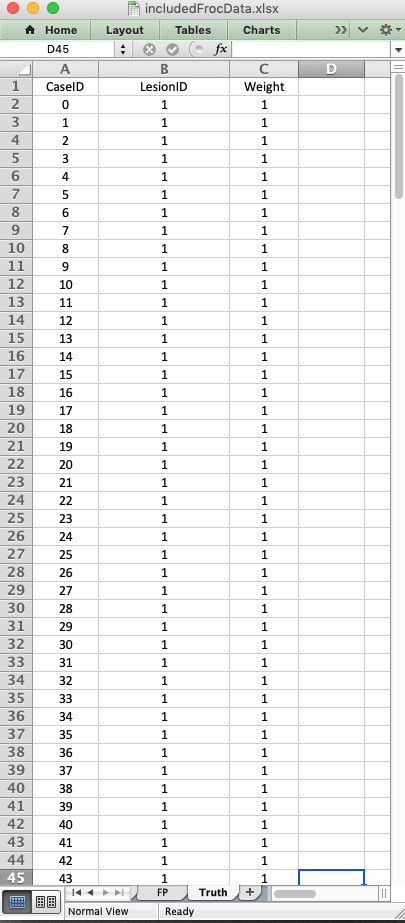
\includegraphics[width=0.4\textwidth,height=\textheight]{images/FROC-Truth-1.png}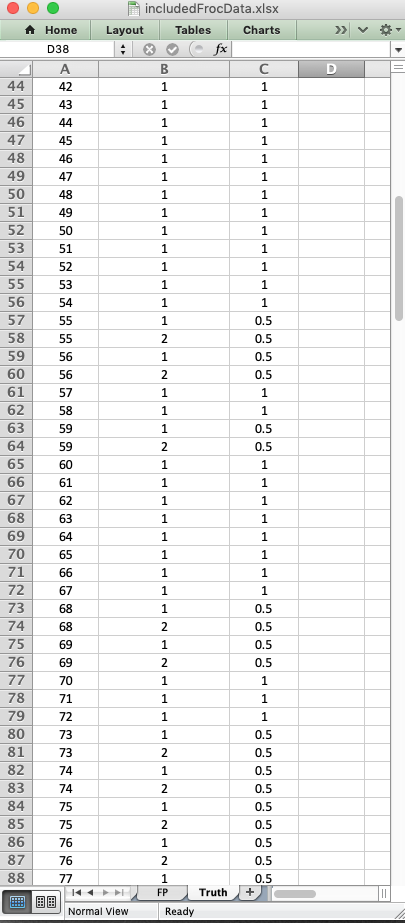
\includegraphics[width=0.4\textwidth,height=\textheight]{images/FROC-Truth-2.png}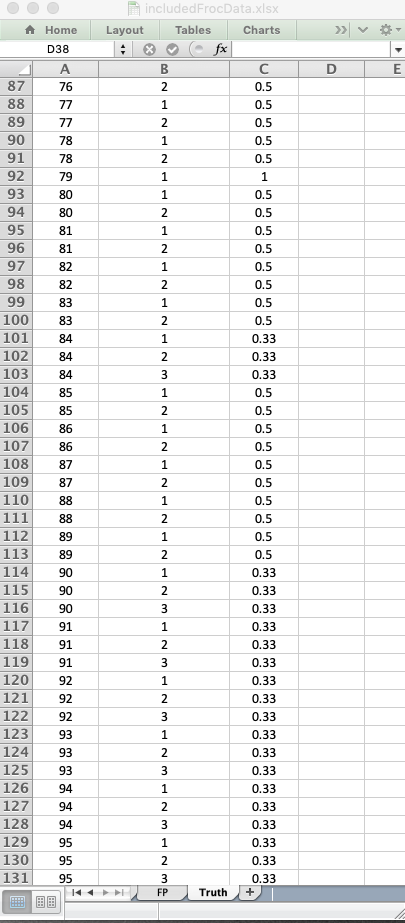
\includegraphics[width=0.4\textwidth,height=\textheight]{images/FROC-Truth-3.png}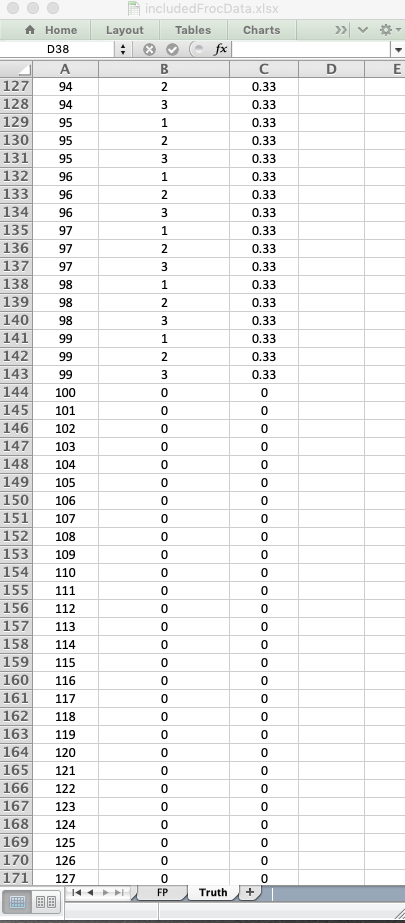
\includegraphics[width=0.4\textwidth,height=\textheight]{images/FROC-Truth-4.png}

\begin{itemize}
\tightlist
\item
  There are 100 diseased cases (labeled 0-99) under column \texttt{CaseID} and 100 non-diseased cases (labeled 100-199). \footnote{The non-diseased cases numbered 128 - 199 are not shown above. They are similar to the ones that are shown - one row per case with a zero under the lesionID column and a zero under the Weights column.}\\
\item
  The \texttt{LesionID} field for each non-diseased case is zero and there is one row per case for such cases. \textbf{For diseased cases, this field has one or more entries, ranging from 1 to 3 for this particular dataset.} In other words, for each diseased case, the number of rows equals the number of lesion on the case.
\item
  As an example, cases labeled \texttt{0\ -\ 54} (and other cases like \texttt{60\ -\ 67}, etc.) have single lesions each, with \texttt{LesionID} = 1 and \texttt{Weight} = 1 have one row per case in the worksheet.
\item
  As another example, there are two rows for \texttt{CaseID} = 77: one with \texttt{LesionID} = 1 (labeling the first lesion on this case) and one with \texttt{LesionID} = 2 (labeling the second and last lesion on this case). The weights of these lesions are explicitly specified as 0.5 each.
\item
  As a final example, there are three rows for \texttt{CaseID} = 95: one with \texttt{LesionID} = 1, one with \texttt{LesionID} = 2 and the last with \texttt{LesionID} = 3. The weights of these lesions are explicitly specified to be 0.33 each. \footnote{The sofware performs a check to ensure that the weight sum to unity, in this case 1\% error is considered close enough for ``government work''!}\\
\item
  Alternatively, the \texttt{Weights} field can be set to zeroes (for all cases) to more conveniently ensure equal weighting to much higher precision.
\item
  Important: every case must have at least one row describing it in the \textbf{Truth} worksheet.
\item
  The Excel files should be ``robust'' with respect to sorting on different columns. By ``robust'' I mean the resulting \texttt{R} dataset object, resulting from \texttt{DfReadDataFile}, should be unchanged. I have not tested this on all files, but if someone brings deviations from this statement to my attention, I will look into it. As a simple example of ``robustness'', notice that in the \textbf{Truth} worksheet being currently explained, the diseased cases come before the non-diseased ones.
\end{itemize}

\hypertarget{the-fpnl-worksheet}{%
\subsection{\texorpdfstring{The \texttt{FP/NL} worksheet}{The FP/NL worksheet}}\label{the-fpnl-worksheet}}

The following screen-shots show different parts of the \texttt{FP} worsheet for \texttt{dataset04}.

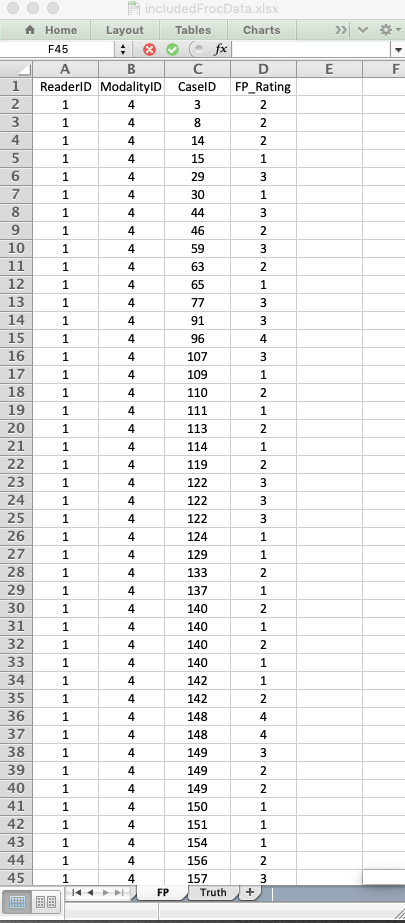
\includegraphics[width=0.4\textwidth,height=\textheight]{images/FROC-FP-1.png}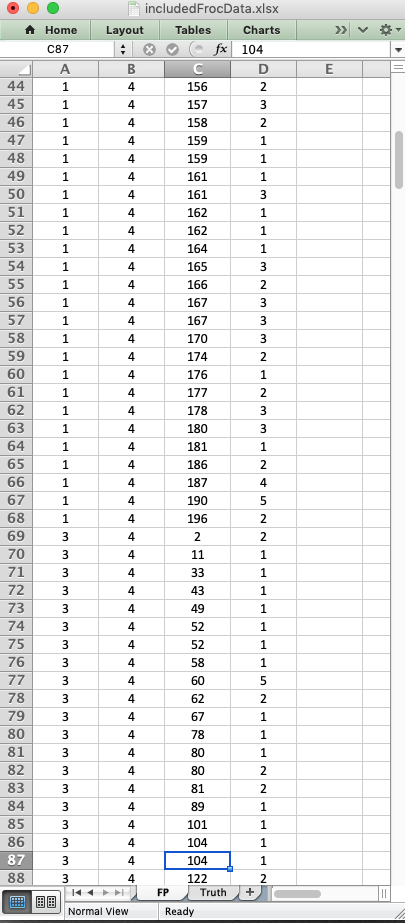
\includegraphics[width=0.4\textwidth,height=\textheight]{images/FROC-FP-2.png}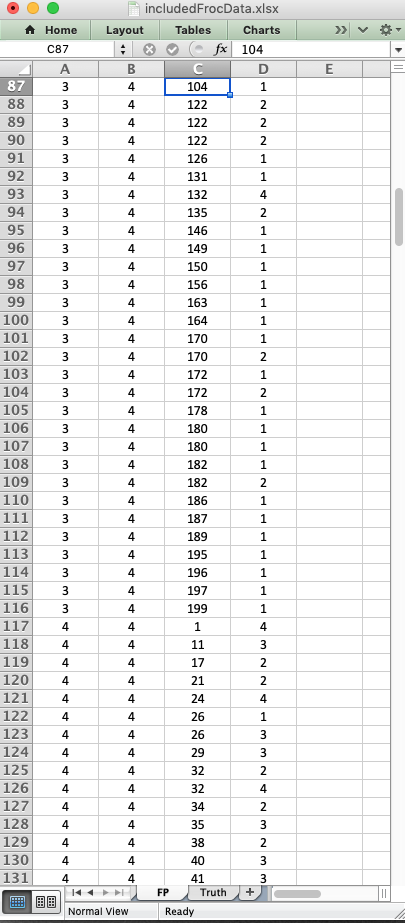
\includegraphics[width=0.4\textwidth,height=\textheight]{images/FROC-FP-3.png}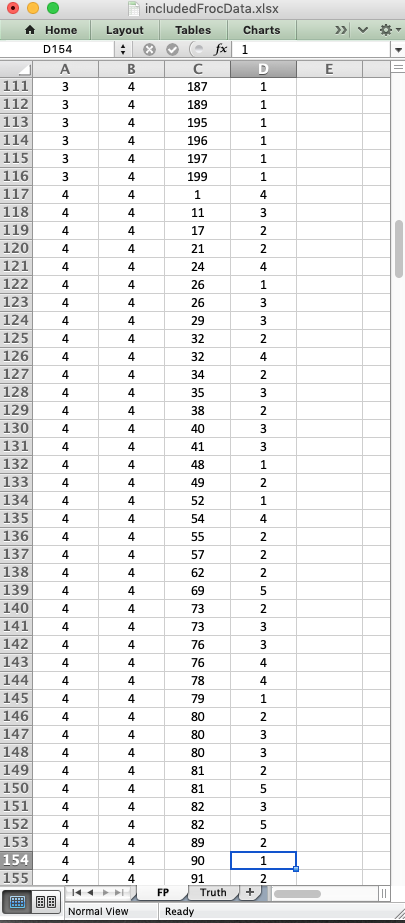
\includegraphics[width=0.4\textwidth,height=\textheight]{images/FROC-FP-4.png}

\begin{itemize}
\tightlist
\item
  The \texttt{FP} worksheet lists the ratings of \texttt{NLs} on both non-diseased and diseased cases. \textbf{Unlike the ROC paradigm, \texttt{NLs} can occur on diseased cases. Additionally, for a given treatment and reader, the number of rows per case cannot be predicted apriori. It could be 0, 1, 2, etc. } While there is in principle no upper limit to the number of \texttt{NLs} per case, radiologists seldom make more than one or two \texttt{NLs} on any case.
\item
  Note the \emph{absence} of the \texttt{LesionID} field. The \texttt{NL} marks do not correspond to real lesions, which by definition, can only occur on diseased cases.
\item
  It is possible (in principle) that the \texttt{FP} worsheet is blank. The observer simplyh does not mark any \texttt{NLs}. See \citep{RN2680} for how the FROC paradigm correctly interprets this situation as indicative of good performance.
\end{itemize}

\hypertarget{the-tpll-worksheet}{%
\subsection{\texorpdfstring{The \texttt{TP/LL} worksheet}{The TP/LL worksheet}}\label{the-tpll-worksheet}}

The following screen-shots show different parts of the \texttt{TP} worsheet for \texttt{dataset04}.

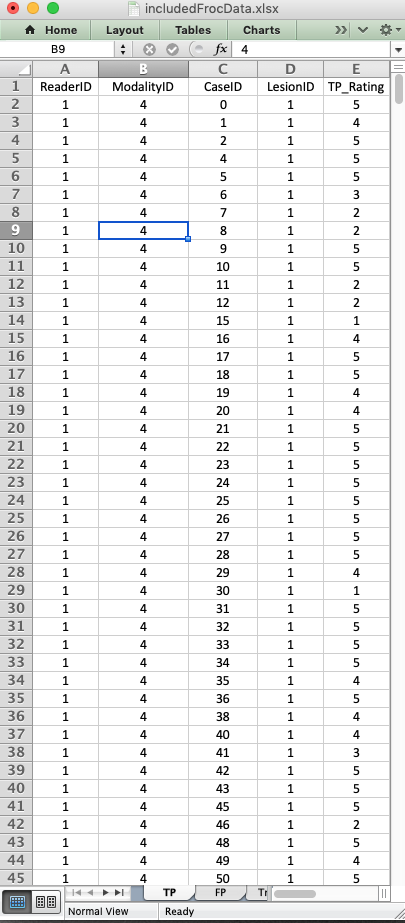
\includegraphics[width=0.4\textwidth,height=\textheight]{images/FROC-TP-1.png}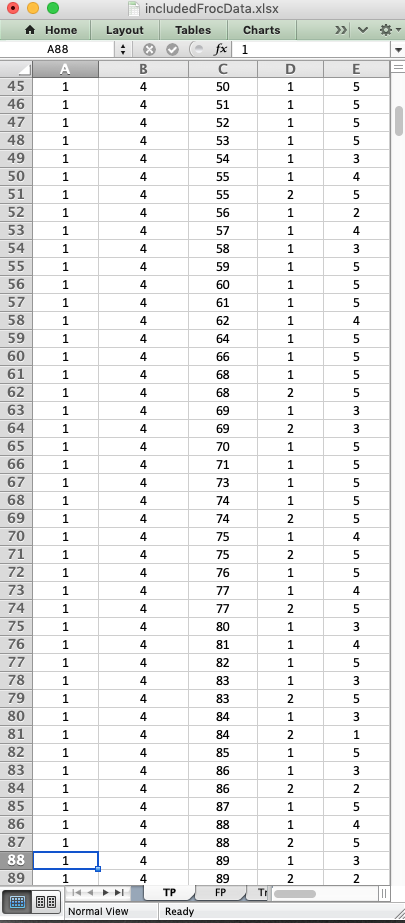
\includegraphics[width=0.4\textwidth,height=\textheight]{images/FROC-TP-2.png}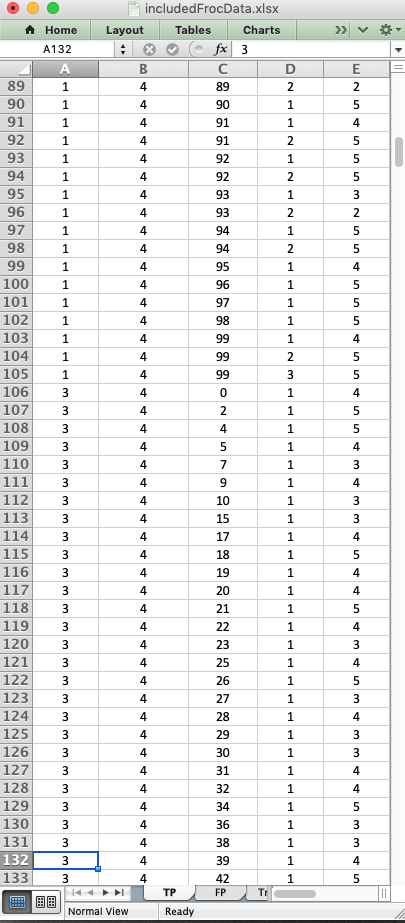
\includegraphics[width=0.4\textwidth,height=\textheight]{images/FROC-TP-3.png}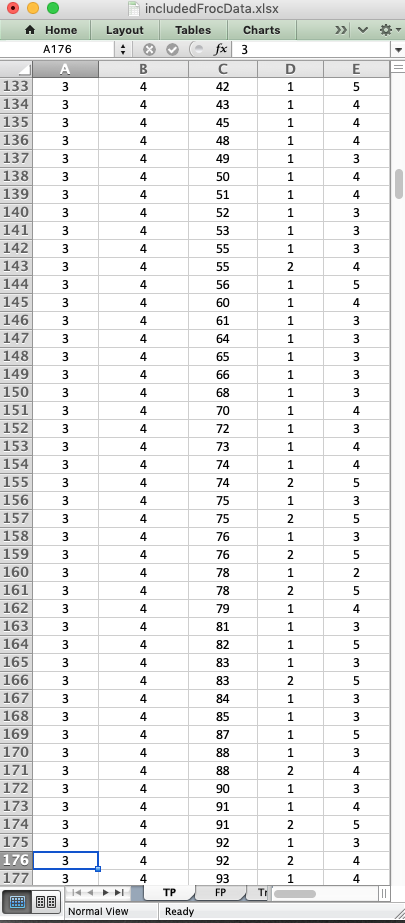
\includegraphics[width=0.4\textwidth,height=\textheight]{images/FROC-TP-4.png}

\begin{itemize}
\tightlist
\item
  The \texttt{TP} worksheet lists the ratings of \texttt{LLs} on diseased cases. \textbf{Only diseased cases can appear on this worksheet. Additionally, for a given treatment and reader, the number of rows per case cannot be predicted apriori. It could be 0, 1, 2, 3} (the upper limit comes from the maximum number of lesions per case in this dataset).
\item
  Note the \emph{presence} of the \texttt{LesionID} field, which essentially names the different lesions on each diseased case.
\item
  As an example, for reader 1, treatment 4, case 99, all three lesions (labeled 1, 2 and 3) are marked and rated 4, 5 and 5, respectively.
\end{itemize}

\begin{Shaded}
\begin{Highlighting}[]
\NormalTok{dataset04}\OperatorTok{$}\NormalTok{lesionID[}\DecValTok{100}\NormalTok{]}
\CommentTok{#> [1] 1}
\NormalTok{dataset04}\OperatorTok{$}\NormalTok{LL[}\DecValTok{4}\NormalTok{, }\DecValTok{1}\NormalTok{, }\DecValTok{100}\NormalTok{, ]}
\CommentTok{#> [1] 4 5 5}
\end{Highlighting}
\end{Shaded}

\begin{itemize}
\tightlist
\item
  The diseased case labeled \texttt{99} in the Excel Truth sheet is actually diseased case number 100 in the \texttt{dataset04\$LL} array.
\item
  Remember that the diseased cases are labeled ``0'' thru ``99'', but the array index in the dataset object runs from 1 to 100.
\item
  As another example, for reader 1, treatment 4, case 3, there are no LL marks. The one lesion on this case went unmarked.
\end{itemize}

\begin{Shaded}
\begin{Highlighting}[]
\NormalTok{dataset04}\OperatorTok{$}\NormalTok{lesionID[}\DecValTok{4}\NormalTok{]}
\CommentTok{#> [1] 1}
\NormalTok{dataset04}\OperatorTok{$}\NormalTok{LL[}\DecValTok{4}\NormalTok{, }\DecValTok{1}\NormalTok{, }\DecValTok{4}\NormalTok{, ]}
\CommentTok{#> [1] -Inf -Inf -Inf}
\end{Highlighting}
\end{Shaded}

\begin{itemize}
\tightlist
\item
  Unmarked lesions are indicated by \texttt{-Inf}.
\item
  It is possible (in principle) that the \texttt{TP} worsheet is blank. See \citep{RN2680} for how the FROC paradigm correctly interprets this situation as indicative of poor performance.
\end{itemize}

\hypertarget{summary-1}{%
\section{Summary}\label{summary-1}}

TBA

\hypertarget{split-plot-analysis}{%
\chapter{Split Plot Analysis}\label{split-plot-analysis}}

\hypertarget{extending-the-dataset-to-accommodate-split-plot-designs}{%
\section{Extending the dataset to accommodate split-plot designs}\label{extending-the-dataset-to-accommodate-split-plot-designs}}

\begin{Shaded}
\begin{Highlighting}[]
\NormalTok{ds <-}\StringTok{ }\NormalTok{dataset02}
\end{Highlighting}
\end{Shaded}

\begin{itemize}
\tightlist
\item
  Need modality index as before.
\item
  Each reader interprets a subset of the cases in both modalities.
\item
  Assume reader \texttt{j} interprets \(K_j\) cases, where K = \(\sum_{i=1}^{J} K_j\) is the total number of cases imaged in both treatments.
\item
  What is the structure of the dataset?
\item
  LL{[}i,j, \(k_j\), 1{]};
\item
  Existing structure should suffice as each case is interpreted twice, once in each treatment, by \emph{only} one reader.
\item
  Assume \texttt{K/J} = integer, 100 in the planned study; \texttt{J} = 8, \texttt{K} = 800
\item
  Modification is needed only in FOM; also dataType needs to be changed to ``SplitPlotRoc'' or ``SplitPlotFroc''
\item
  ROC\_SP or FROC\_SP
\item
  LL{[}i,j, 800, 1{]} for ROC
\item
  LL{[}i,j, 800, maxL{]} for FROC
\item
  Likewise for NL arrays
\item
  Work next on FOM
\item
  git commit -m `documentation update {[}ci skip{]}'
\end{itemize}

\hypertarget{introduction-2}{%
\section{Introduction}\label{introduction-2}}

Jason:
Thanks for inviting me to join your profile. Could you describe what you were planning on doing? Please use a simple example that illustrates the basic data collection. The key ~point I want to be sure about is that strict pairing of readers across different treatments is preserved. I once had a study that had different readers interpreting in different treatments, which makes it impossible to separate the treatment effect (which is our primary interest) from a treatment-reader interaction effect. I am going to post that problem on Research Gate (the regulatory agency was telling them to do the study in a non-scientific way). Dev

Dr.~Chakraborty, there will be 8 readers in my study. Around 800 CT images will be collected. Each reader reads 100 CT images unaided and aided by the CADe in two independent reading sessions separated by a washout period of 4 weeks. Each CT image will only be interpreted by one reader. I think it is a split-plot design with cases nested within reader so the strict pairing of readers across different treatments is preserved. Thanks for your help!

Hi Jason,
This problem has been solved in the ROC context (localization information not used) by Hillis and others; they may even have software. To analyze it using localization, one needs to use a location-sensitive figure of merit, like the weighted AFROC. That would be my recommendation. So, for each reader j, one has a figure of merit theta\_ij, where i is the modality index. One can average over j, yielding theta\_i\_dot. Significance testing can be performed in the usual manner - e.g., DBMH or ORH. A custom program would need to be written or one can construct one out of R-scripts using the existing functions in RJafroc (the Windows program is obsolete). I can help in this regard. I would ask you to read the relevant papers and explain to me if my approach, summarized above, is basically correct. In any case, any method for ROC analysis can be adapted to FROC analysis if one uses the appropriate figure of merit. Good luck. Dev

Jason: Attached is the Hillis paper; I am not a statistician and find the term ``nested'' confusing; this paper claims to analyze split plot design using the OR approach as applied to ROC split plot data; if you think this is the correct approach for your study, apart from the limitation to ROC, I can easily extend the software to analyze FROC split plot data; please review and advise; Dev

\hypertarget{roidataformat}{%
\chapter{ROI data format}\label{roidataformat}}

\hypertarget{roi-paradigm}{%
\section{ROI paradigm}\label{roi-paradigm}}

\begin{itemize}
\tightlist
\item
  One can think of the ROI paradigm as similar to the FROC paradigm, but with localization accuracy restricted to belonging to a region (one cannot distinguish multiple lesions within a region). The ROIs are defined prior to the study and made known to all observers participating in the study. Unlike the FROC paradigm, a \textbf{rating is required for every ROI}.
\end{itemize}

\bibliography{packages.bib,myRefs.bib}


\end{document}
